\documentclass[11pt,a4paper,reqno]{amsart}

\usepackage[utf8]{inputenc}
\usepackage[T1]{fontenc}
\usepackage{amsmath,amssymb,amsthm,mathtools}
\usepackage{booktabs}
\usepackage{graphicx}
\usepackage{enumitem}
\usepackage{xcolor}
\usepackage{microtype}
\usepackage[hidelinks]{hyperref}
\usepackage[capitalise,noabbrev]{cleveref}

\setlength{\textwidth}{6.2in}
\setlength{\oddsidemargin}{0.14in}
\setlength{\evensidemargin}{0.14in}
\setlength{\textheight}{9.0in}
\setlength{\topmargin}{-0.2in}
\emergencystretch=1.5em

\newtheorem{theorem}{Theorem}[section]
\newtheorem{proposition}[theorem]{Proposition}
\newtheorem{lemma}[theorem]{Lemma}
\newtheorem{corollary}[theorem]{Corollary}
\theoremstyle{definition}
\newtheorem{definition}[theorem]{Definition}
\newtheorem{assumption}[theorem]{Assumption}
\theoremstyle{remark}
\newtheorem{remark}[theorem]{Remark}

\newcommand{\R}{\mathbb{R}}
\newcommand{\E}{\mathbb{E}}
\newcommand{\Var}{\mathrm{Var}}
\newcommand{\Prob}{\mathbb{P}}
\newcommand{\Ncal}{\mathcal{N}}
\newcommand{\Xcal}{\mathcal{X}}
\newcommand{\dd}{\mathrm{d}}
\newcommand{\tr}{\mathrm{tr}}

\title[Design-Time Learning-Rate Selection for GBOED]{Design-Time Learning-Rate Selection and Dispersion-Gated Tempering for Generalised Bayesian Experimental Design}

\author{Thijs Missiaen}
\address{Independent Researcher, Belgium}
\email{thijs.missiaen@gmail.com}

\date{\today}

\begin{document}

\begin{abstract}
We solve design-time learning-rate selection for generalised Bayesian optimal experimental design (GBOED) under predictive-centered inverse multi-quadric weighted score matching (PredC IMQ-WSM). Our method certifies homoscedasticity and design-invariance from prior simulator draws, derives the exact calibration ratio $\omega_0(c)/\sigma^2 = H_B/J_B$ in $\mathbb{R}^p$ via Stein's identity and 50-digit ball quadrature, and modulates $\omega_t$ online via standardized prior-data conflict $\hat{\Delta}_0^2$ and posterior-predictive dispersion $S_t^{\mathrm{pred}}$ without peeking at data-generating scenarios. We prove uniform rate bounds, bounded influence iff $p_{\mathrm{IMQ}} \ge 1/2$, asymptotic tail unbiasedness iff $p_{\mathrm{IMQ}} > 1/2$, Huber contamination bounds, consistency, asymptotic Godambe covariance, and finite-sample NLL vs.\ sample-pair MSE tradeoffs, while showing that variance-heteroscedastic models retain a finite tail gap preventing scalar calibration. Across nine sequential benchmark scenarios ($R=90$ to $270$), a single frozen rule matches standard BOED when well specified and lowers both MMD and NLL by $-2.23$ to $-10.75$ unpaired standard errors under outliers and noise misspecification.
\end{abstract}

\maketitle

\section{Introduction}\label{sec:intro}

In sequential Bayesian optimal experimental design (BOED), experimenters iteratively select designs $\xi_t \in \Xcal$ by maximizing expected information gain (EIG)~\cite{lindley1956measure,rainforth2024modern,overstall2020acebayes}. Because exact Kullback--Leibler posteriors concentrate around misspecified pseudo-true parameters~\cite{grunwald2017inconsistency} and break down under contaminated responses, generalized Bayesian updating replaces log-likelihoods with a loss function $\ell$ weighted by a learning rate $\omega > 0$~\cite{bissiri2016general,knoblauch2022optimization,jewson2022loss}. At horizon $t$, GatedC G-LHW forms the batch-reweighted generalized posterior using the active scalar pair $(\omega_t, c_t)$:
\[
\pi_t^{\omega_t, c_t}(\theta) \propto \pi(\theta)\exp\!\Bigl(-\omega_t \sum_{j=1}^t \ell_B(\theta; y_j, \xi_j; \hat{\mu}_{t,j}, c_t)\Bigr).
\]
Calibration of $\omega$ without holdout tuning has been studied for general updating~\cite{lyddon2019general,wu2023comparison,grunwald2017inconsistency}, and score-matching divergences~\cite{hyvarinen2005score,barp2019minimum} with inverse multi-quadric (IMQ) weights yield bounded-influence generalized posteriors~\cite{altamirano2024rcgp,laplante2025strcgp}. Recently, Barlas, Sloman, and Kaski~\cite{barlas2025gboed} extended this paradigm to GBOED using predictive-centered IMQ weighted score matching (PredC IMQ-WSM), defined for a fixed centering scalar $\hat{\mu} \in \R$, threshold $c > 0$, and Gaussian simulator $p(y \mid \theta, \xi) = \Ncal(y; \mu_\theta(\xi), \sigma_\theta(\xi)^2)$ with weight $m(y; \hat{\mu}, c) = (1 + (y - \hat{\mu})^2 / c^2)^{-p_{\mathrm{IMQ}}/2}$ ($p_{\mathrm{IMQ}} > 0$) by
\begin{equation}\label{eq:predc_loss_def}
\ell_B(\theta; y, \xi; \hat{\mu}, c)
= m(y; \hat{\mu}, c)^2 s_\theta(\xi, y)^2 + 2\Bigl(m(y; \hat{\mu}, c)^2 \partial_y s_\theta(\xi, y) + \partial_y\bigl[m(y; \hat{\mu}, c)^2\bigr]\,s_\theta(\xi, y)\Bigr),
\end{equation}
where $s_\theta(\xi, y) = \partial_y \log p(y \mid \theta, \xi) = (\mu_\theta(\xi) - y)/\sigma_\theta(\xi)^2$. Selecting $(\omega_t, c_t)$ prior to data collection using only design-time inputs $(\pi, p(y \mid \theta, \xi), \ell_B, \Xcal)$ and within-experiment history remains an open problem. In particular, arbitrary exponential decay schedules heuristically tuned per task fail to transfer across noise scales, while naive unannealed IMQ centering collapses under severe prior-data conflict.

We provide a principled design-time and online rule, \emph{GatedC G-LHW}, whose constants are derived analytically at $p_{\mathrm{IMQ}} = 1$ using 50-digit \texttt{python-flint} \texttt{arb} ball quadrature:
\begin{equation}\label{eq:constants_decl}
\begin{aligned}
\frac{\omega_0(2\sigma)}{\sigma^2} &\in [0.530512267190, 0.530512267191], &
\sup_{z\in\R}|\psi_B(z; 2, 1)| &= 1.273875757928\dots,\\
\frac{\omega_0(5\sigma)}{\sigma^2} &\in [0.515066297315, 0.515066297316], &
\sup_{z\in\R}|\psi_B(z; 5, 1)| &= 2.601919536104\dots,\\
\omega_t &\in \bigl[0.128766574328\sigma^2,\, 1.061024534381\sigma^2\bigr], &
\gamma_\infty &\in [0.25,\, 2.0].
\end{aligned}
\end{equation}

\begin{theorem}[Main Calibration, Robustness, and Structural Separation Theorem]\label{thm:main}
Let $p(y \mid \theta, \xi) = \Ncal(y; \mu_\theta(\xi), \sigma_\theta(\xi)^2)$ with known prior $\pi(\theta)$ on $\Theta \subseteq \R^p$ and design space $\Xcal$. Let $\ell_B$ be the PredC IMQ-WSM loss~\eqref{eq:predc_loss_def}.
\begin{enumerate}[label=(\alph*)]
\item \textbf{Design-time separation (\cref{thm:heteroscedastic}).} Scalar learning-rate selection via $\ell_B$ preserves asymptotic tail unbiasedness ($\Delta_\infty(\xi) = 0$) when $\sigma_\theta(\xi) \equiv \sigma$ is both $\theta$-independent and $\xi$-constant provided $p_{\mathrm{IMQ}} > 1/2$, whereas on non-constant means $\mu_\theta(\xi)$, $p_{\mathrm{IMQ}} = 1/2$ leaves a finite plateau $\Delta_\infty(\xi) > 0$ and $0 < p_{\mathrm{IMQ}} < 1/2$ diverges ($\Delta_\infty(\xi) = +\infty$). When $\sigma_\theta(\xi)$ is $\theta$-dependent and $p_{\mathrm{IMQ}} = 1$, $\ell_B(\theta; y, \xi) \to c(\xi)^2 / \sigma_\theta(\xi)^4$ as $|y|\to\infty$, creating a finite strictly positive variance tail gap $\Delta_\infty(\xi) \in (0, 100 c(\xi)^2]$ on pharmacokinetic variance laws $\sigma_\theta(\xi) = (0.01\mu_\theta(\xi)^2 + 0.1)^{1/2}$ that biases outliers toward larger predictive variance.
\item \textbf{Multivariate Stein calibration (\cref{prop:stein_fisher,cor:multivariate_lhw}).} Under homoscedastic noise $\sigma_\theta(\xi) \equiv \sigma$, for every fixed $\hat{\mu} \in \R$, Stein's identity makes the natural-mean score $\partial_\mu \ell_B(\mu^*; Y)$ Fisher consistent under $Y \sim \Ncal(\mu^*, \sigma^2)$ with positive curvature $\partial_\mu^2 \ell_B > 0$. The influence function $\psi_B$ is uniformly bounded if and only if $p_{\mathrm{IMQ}} \ge 1/2$, and for $p_{\mathrm{IMQ}} = 1$ all $p$-dimensional Fisher matrix factors cancel in the Lyddon--Walker--Holmes identity $(\omega_0\bar{H}_T)^{-1} = \bar{H}_T^{-1}\bar{J}_T\bar{H}_T^{-1}$, yielding $\omega_0(c) = \sigma^2 H_B(c/\sigma) / J_B(c/\sigma)$.
\item \textbf{Gated online guarantees and experimental performance (\cref{thm:gatedc_guarantees,thm:conflict_floor}).} Under the frozen GatedC G-LHW gate using pure-Bayesian annealed continuation in conjugate linear models (or sequential predictive centering in nonlinear SMC), the learning rate lies unconditionally in $[0.25\,\omega_0(5\sigma),\, 2\,\omega_0(2\sigma)]$, posterior parameter shift under arbitrary single-point contamination stays uniformly bounded, the M-estimator is consistent under well-specified and symmetric $\varepsilon$-contaminated models, and the limiting Gibbs covariance equals $T^{-1}\gamma_\infty^{-1}\bar{H}_T(c_T)^{-1}\bar{J}_T(c_T)\bar{H}_T(c_T)^{-1}(1 + o_p(1))$ with $\gamma_\infty \in [0.25, 2]$. Evaluated over nine benchmark scenarios ($R \in \{90, 270\}$), the identical rule improves over BOED by $-2.23$ to $-10.75$ unpaired standard errors ($-2.68$ to $-18.60$ paired) on MMD and NLL under outliers and noise misspecification without degradation on well-specified models.
\end{enumerate}
\end{theorem}

\subsection{Proof overview}\label{sec:overview}
The proof of \cref{thm:main} combines three quantitative and structural ingredients that cleanly separate exact mathematics from frozen algorithm choices:
\begin{enumerate}[label=\arabic*.]
\item \emph{Exact score geometry and heteroscedastic obstruction} (\cref{sec:theory}): Differentiating~\eqref{eq:predc_loss_def} cleanly in $\mu$ shows that $\ell_B$ is linear plus quadratic in $\mu$ with $y$-dependent weights $m^2$ and $(m^2)'$. Gaussian integration by parts eliminates bias at $\mu^*$ independently of $\hat{\mu}$, collapses multivariate $\R^p$ sandwich matrices onto $\bar{G}_T$, proves bounded influence iff $p_{\mathrm{IMQ}} \ge 1/2$, and exposes the finite tail gap $\Delta_\infty(\xi)$ under $\theta$-dependent variance.
\item \emph{Prior-conflict geometry and pure-Bayesian continuation} (\cref{sec:theory,sec:algorithm}): Exact 1D conjugate closed forms establish why $\omega < 1$ amplifies prior bias, why $\partial_u \E[\mathrm{NLL}]|_{u=0}$ and $\partial_u \E[\mathrm{MSE}_{\mathrm{pred}}]|_{u=0}$ can have opposite signs when $T > 2 r_0 \kappa$, and why deterministic five-step continuation avoids IMQ center collapse without ad-hoc estimators.
\item \emph{Huber contamination and large-sample Godambe calibration} (\cref{sec:theory,sec:benchmarks}): Uniformly bounding $\psi_B$ controls the influence of unbounded outliers on both generalized scores and conjugate normal equations, while stochastic domination $S_t^{\mathrm{pred}} \preceq_{\mathrm{st}} \chi^2_t$ keeps the dispersion gate inactive under well-specified sampling and activates downweighting under overdispersion.
\end{enumerate}
Together, Ingredients 1 and 2 establish exact well-specified calibration and conflict relief, while Ingredient 3 certifies robustness and empirical performance across sequential adaptive designs.

\subsection{Notation and conventions}\label{sec:notation}
Throughout, $Y_t \in \R$ denotes the $t$-th response at design $\xi_t \in \Xcal$, observed from an unknown data-generating distribution $P^*(\cdot \mid \xi_t)$ with simulator $p(y \mid \theta, \xi) = \Ncal(y; \mu_\theta(\xi), \sigma_\theta(\xi)^2)$ parameterized by $\theta \in \Theta \subseteq \R^p$ under prior $\pi(\theta) = \Ncal(\theta; \mu_0, \Sigma_0)$ (or precision $\Sigma_0^{-1} = P_0$). For $c > 0$ and $p_{\mathrm{IMQ}} > 0$, set $m(y; \hat{\mu}, c) = (1 + (y - \hat{\mu})^2 / c^2)^{-p_{\mathrm{IMQ}}/2}$ and denote the standardized kernel weight by $m_0(z; r, p_{\mathrm{IMQ}}) = (1 + z^2 / r^2)^{-p_{\mathrm{IMQ}}/2}$ with $r = c/\sigma$. Given posterior draws $\theta^{(1)}, \dots, \theta^{(M)}$ from a generalized posterior $q_t$, predictive mean and epistemic variance at design $\xi$ are $\hat{\mu}_t(\xi) = M^{-1}\sum_{m=1}^M \mu_{\theta^{(m)}}(\xi)$ and $\hat{\sigma}_{\mathrm{ep}, t}^2(\xi) = M^{-1}\sum_{m=1}^M (\mu_{\theta^{(m)}}(\xi) - \hat{\mu}_t(\xi))^2$. Because benchmark methods are evaluated across coupled replicate streams of length $R$ sharing identical true parameters $\theta^*_r$, prior noise draws, and clean observation seeds, we report conservative unpaired standardized effects
\[
z_{\mathrm{uSE}} = \frac{\bar{M}_A - \bar{M}_B}{\sqrt{\mathrm{SE}_A^2 + \mathrm{SE}_B^2}},
\]
where $\mathrm{SE}_A = \hat{s}_A / \sqrt{R}$ (negative $z_{\mathrm{uSE}}$ favors method $A$ on RMSE, kernel MMD$^2$, and predictive NLL), together with paired standardized effects $z_{\mathrm{pSE}} = (\bar{M}_A - \bar{M}_B)/\mathrm{SE}(M_{A,1:R} - M_{B,1:R})$ where cross-method pairings are compared explicitly.

We maintain a strict three-layer separation across \cref{sec:theory,sec:algorithm,sec:benchmarks}: unconditional theorems and exact algebraic identities appear first, conditional propositions list every hypothesis explicitly in their statement headers, and engineering hyperparameters plus finite-sample numerical audits are isolated from formal proofs.

\section{Structural Theory and Asymptotic Calibration}\label{sec:theory}

\subsection{Design-time homoscedasticity criterion and pharmacokinetic obstruction}

\begin{definition}[Relative variation and asymptotic tail gap]\label{def:variations}
For a design-time grid $\Theta_0 = \{\theta_k\}_{k=1}^K \sim \pi$ and $\Xcal_0 = \{\xi_d\}_{d=1}^D \subset \Xcal$ with $K, D \ge 2$, define the $\theta$-heteroscedasticity ratio, design-wise scale variation, and asymptotic tail gap at fixed centering $\hat{\mu} \in \R$ and $c(\xi) > 0$ by
\begin{align*}
\rho_\theta &= \max_{1 \le d \le D} \frac{\max_k \sigma_{\theta_k}(\xi_d) - \min_k \sigma_{\theta_k}(\xi_d)}{\min_k \sigma_{\theta_k}(\xi_d)}, \\
\rho_\xi &= \frac{\max_d \mathrm{med}_k \sigma_{\theta_k}(\xi_d) - \min_d \mathrm{med}_k \sigma_{\theta_k}(\xi_d)}{\min_d \mathrm{med}_k \sigma_{\theta_k}(\xi_d)}, \\
\Delta_\infty(\xi) &= \sup_{\theta_1, \theta_2 \in \Theta} \lim_{|y| \to \infty} \bigl|\ell_B(\theta_1; y, \xi; \hat{\mu}, c(\xi)) - \ell_B(\theta_2; y, \xi; \hat{\mu}, c(\xi))\bigr|.
\end{align*}
\end{definition}

\begin{theorem}[Tail Gap Separation and Finite Pharmacokinetic Bound]\label{thm:heteroscedastic}
Let $p(y \mid \theta, \xi) = \Ncal(y; \mu_\theta(\xi), \sigma_\theta(\xi)^2)$ with $\sigma_\theta(\xi) > 0$ and bounded $\mu_\theta(\xi)$ at each fixed $\xi \in \Xcal$ and $c(\xi) > 0$.
\begin{enumerate}[label=(\alph*)]
\item \textbf{Homoscedastic vanishing threshold ($p_{\mathrm{IMQ}} > 1/2$).} If $\sigma_\theta(\xi) \equiv \sigma$ is constant in $(\theta, \xi)$, then $\Delta_\infty(\xi) = 0$ for every $p_{\mathrm{IMQ}} > 1/2$. When $\sup_{\theta_1, \theta_2 \in \Theta}|\mu_{\theta_1}(\xi) - \mu_{\theta_2}(\xi)| > 0$, the critical exponent $p_{\mathrm{IMQ}} = 1/2$ yields a finite positive plateau $\Delta_\infty(\xi) = 2 c(\xi)\sigma^{-4}\sup_{\theta_1,\theta_2 \in \Theta}|\mu_{\theta_1}(\xi) - \mu_{\theta_2}(\xi)| > 0$, while $0 < p_{\mathrm{IMQ}} < 1/2$ gives $\Delta_\infty(\xi) = +\infty$.
\item \textbf{Finite positive PK tail gap at $p_{\mathrm{IMQ}} = 1$.} For $p_{\mathrm{IMQ}} = 1$ and arbitrary $\hat{\mu} \in \R$,
\[
\lim_{|y| \to \infty} \ell_B(\theta; y, \xi; \hat{\mu}, c(\xi)) = \frac{c(\xi)^2}{\sigma_\theta(\xi)^4}, \qquad
\Delta_\infty(\xi) = c(\xi)^2\Bigl(\sup_{\theta \in \Theta} \sigma_\theta(\xi)^{-4} - \inf_{\theta \in \Theta} \sigma_\theta(\xi)^{-4}\Bigr).
\]
In the pharmacokinetic model $\sigma_\theta(\xi) = (0.01 \mu_\theta(\xi)^2 + 0.1)^{1/2} \ge \sqrt{0.1}$ with $p_{\mathrm{IMQ}} = 1$, $\Delta_\infty(\xi)$ is finite and strictly positive with $0 < \Delta_\infty(\xi) \le 100 c(\xi)^2$ whenever $\mu_\theta(\xi)^2$ varies across $\theta \in \Theta$, favoring larger-variance parameters $\theta$ on gross outliers regardless of location error.
\item \textbf{Residual-scale persistence for $p_{\mathrm{IMQ}} > 1$.} If $p_{\mathrm{IMQ}} > 1$, then $\lim_{|y|\to\infty}\ell_B(\theta; y, \xi) = 0$ ($\Delta_\infty(\xi) = 0$); yet at any finite outlier $r = y - \hat{\mu}$ with $u = 1 + r^2/c(\xi)^2 > 1$, score-matching likelihood differences $\ell_B(\theta_1; y, \xi) - \ell_B(\theta_2; y, \xi)$ remain non-vanishing on moderate outliers $|r| = \mathcal{O}(c(\xi))$, obstructing variance-unbiased scalar weighting.
\end{enumerate}
\end{theorem}

Audit measurements (\texttt{results/audit\_results.json}) illustrate \cref{thm:heteroscedastic} directly on Barlas's pharmacokinetic simulator~\cite{barlas2025gboed}: prior draws give $\rho_\theta = 2.5013$, prior-grid lower bound $\Delta_\infty \ge 71.5635$, and prior-grid upper bound $\max_{\xi \in \Xcal_0} 100 c(\xi)^2 = 949.3513$ (rising to $100 c_{\mathrm{pk}}^2 = 1716.9020$ at evaluation design $\xi = 2\,\mathrm{h}$, $c_{\mathrm{pk}} = 2\sigma^* = 4.1436$). At $\xi = 2\,\mathrm{h}$, comparing $\theta^*$ ($\sigma^* = 2.0718$) against $\theta_{\mathrm{alt}}$ ($\sigma_{\mathrm{alt}} = 3.5006$), the $p_{\mathrm{IMQ}} = 1$ tail loss converges from $0.8966$ at $y=5$ to $0.931911 \approx c_{\mathrm{pk}}^2/(\sigma^*)^4$ at $y=10^4$ for $\theta^*$, versus $0.114011 \approx 0.114340 = c_{\mathrm{pk}}^2/\sigma_{\mathrm{alt}}^4$ for $\theta_{\mathrm{alt}}$ (\cref{fig:pk_ablation}(a)). Even at $p_{\mathrm{IMQ}} = 2$ where $|\ell_B| \to 0$ in the far tail ($1.61 \times 10^{-7}$ at $y=10^4$), the moderate negative residual $y - \hat{\mu} = -5$ yields a bias gap of $0.5221$ ($0.9657$ at $p_{\mathrm{IMQ}} = 1$). On homoscedastic draws confirming part~(a), prior-centered tail differences $\Delta y \in \{10^2, 10^4, 10^6\}$ grow as $\{28.14, 282.83, 2828.43\}$ for $p_{\mathrm{IMQ}} = 0.25$, plateau at $4.0$ ($3.9796 \to 3.999998$) for $p_{\mathrm{IMQ}} = 0.5$, and decay as $\{0.0796, 8\times 10^{-4}, 8\times 10^{-6}\}$ for $p_{\mathrm{IMQ}} = 1$. Consequently, GatedC G-LHW certifies $\rho_\theta \le 10^{-6}$ and $\rho_\xi \le 10^{-6}$ at design time and declines automatic scalar operation on non-certified heteroscedastic models, $\xi$-varying noise, or $p_{\mathrm{IMQ}} \le 1/2$.

\subsection{Stein Fisher consistency, bounded influence, and multivariate LHW ratio}

\begin{proposition}[Stein Fisher Consistency and Redescending Influence Bound]\label{prop:stein_fisher}
Assume $p(y \mid \mu, \sigma) = \Ncal(y; \mu, \sigma^2)$ with known constant $\sigma > 0$, threshold $c = r\sigma > 0$, $p_{\mathrm{IMQ}} > 0$, and arbitrary fixed centering scalar $\hat{\mu} \in \R$. Define
\[
\psi_B(z; r, p_{\mathrm{IMQ}}) = z\Bigl(1 + \frac{z^2}{r^2}\Bigr)^{-p_{\mathrm{IMQ}}} + \frac{2 p_{\mathrm{IMQ}} z}{r^2}\Bigl(1 + \frac{z^2}{r^2}\Bigr)^{-p_{\mathrm{IMQ}}-1},
\]
and the dimensionless quadrature functionals under $Z \sim \Ncal(0, 1)$,
\[
H_B(r, p_{\mathrm{IMQ}}) = 2\,\E\bigl[m_0(Z; r, p_{\mathrm{IMQ}})^2\bigr], \qquad
J_B(r, p_{\mathrm{IMQ}}) = 4\,\E\bigl[\psi_B(Z; r, p_{\mathrm{IMQ}})^2\bigr].
\]
\begin{enumerate}[label=(\alph*)]
\item \textbf{Universal Stein Fisher consistency.} For every $\hat{\mu} \in \R$ (even $\hat{\mu} \neq \mu^*$),
\[
\E_{Y \sim \Ncal(\mu^*, \sigma^2)}\bigl[\partial_\mu \ell_B(\mu^*; Y; \hat{\mu}, c)\bigr] = 0.
\]
\item \textbf{Uniform strict convexity.} For every $\mu, y, \hat{\mu} \in \R$, $\partial_\mu^2 \ell_B(\mu; y; \hat{\mu}, c) = \frac{2}{\sigma^4} m(y; \hat{\mu}, c)^2 > 0$. Evaluating at $\hat{\mu} = \mu^*$ yields $\E[\partial_\mu^2 \ell_B(\mu^*; Y)] = H_B / \sigma^4$ and $\E[(\partial_\mu \ell_B(\mu^*; Y))^2] = J_B / \sigma^6$.
\item \textbf{Boundedness criterion and exact radical.} We have $\sup_{z \in \R} |\psi_B(z; r, p_{\mathrm{IMQ}})| < \infty$ if and only if $p_{\mathrm{IMQ}} \ge 1/2$. For $p_{\mathrm{IMQ}} = 1$, the unique positive maximizer is $z_*(r) = r w_*(r)$ where $w_*(r) = \bigl(\sqrt{9r^{-4} + 2r^{-2} + 1} - 3r^{-2}\bigr)^{1/2}$ solves $w^4 + 6r^{-2}w^2 - (1 + 2r^{-2}) = 0$.
\end{enumerate}
\end{proposition}

Fifty-digit interval quadrature via \texttt{flint.arb} (\cref{tab:quadrature}) matches \texttt{scipy.integrate.quad} within $1.33 \times 10^{-15}$, while numerical Stein expectation checks across shifts $\hat{\mu} - \mu^* \in [-10\sigma, +8\sigma]$ vanish to $\le 2.05 \times 10^{-16}$. The Godambe efficiency index $H_B^2 / J_B$ stays close to unity ($0.8942$ at $r=2$ and $0.9931$ at $r=5$ for $p_{\mathrm{IMQ}}=1$), showing minimal asymptotic Fisher information loss relative to Gaussian maximum likelihood.

\begin{table}[t]
\centering
\small
\caption{Certified 50-digit \texttt{flint.arb} Gaussian quadrature constants for PredC IMQ-WSM at threshold ratio $r = c/\sigma$ and kernel exponent $p_{\mathrm{IMQ}}$ (all \texttt{arb} interval radii $\le 4.94 \times 10^{-22}$).}\label{tab:quadrature}
\begin{tabular}{@{}cccccc@{}}
\toprule
$p_{\mathrm{IMQ}}$ & $r = c/\sigma$ & $H_B$ & $J_B$ & $\omega_0 / \sigma^2 = H_B/J_B$ & $H_B^2/J_B$ \\
\midrule
$1$ & $2$ & $1.6854769172$ & $3.1770743513$ & $0.5305122672$ & $0.8941661806$ \\
$1$ & $5$ & $1.9280810472$ & $3.7433648002$ & $0.5150662973$ & $0.9930895659$ \\
$2$ & $2$ & $1.4717846243$ & $2.9952949851$ & $0.4913655021$ & $0.7231841909$ \\
$2$ & $5$ & $1.8630274342$ & $3.5581655356$ & $0.5235921195$ & $0.9754664829$ \\
\bottomrule
\end{tabular}
\end{table}

\begin{corollary}[Multivariate LHW Matrix Alignment in $\R^p$]\label{cor:multivariate_lhw}
Suppose $\sigma_\theta(\xi) \equiv \sigma$ is constant on $\Theta \times \Xcal$, $p_{\mathrm{IMQ}} \ge 1/2$, sequential designs $\xi_j$ are predictable ($\mathcal{F}_{j-1}$-measurable, with $\mathcal{F}_{j-1} = \sigma(\xi_1, Y_1, \dots, \xi_{j-1}, Y_{j-1}, \xi_j)$) and observations satisfy $Y_j \mid \mathcal{F}_{j-1} \sim \Ncal(\mu_{\theta^*}(\xi_j), \sigma^2)$, the mean map $\theta \mapsto \mu_\theta(\xi)$ is $C^2$ near $\theta^* \in \mathrm{int}(\Theta)$ with uniformly bounded derivatives $\|\nabla_\theta\mu_{\theta^*}(\xi)\|_2 \le L_\mu$ and $\|\nabla_\theta^2\mu_{\theta^*}(\xi)\|_{\mathrm{op}} \le K_\mu$ over $\Xcal$, designs yield $\bar{G}_T = T^{-1}\sum_{j=1}^T \nabla_\theta \mu_{\theta^*}(\xi_j)\nabla_\theta \mu_{\theta^*}(\xi_j)^\top \succeq \lambda_{\min} I_p \succ 0$, and centerings satisfy $\max_{1\le j\le T}|\hat{\mu}_{T,j} - \mu_{\theta^*}(\xi_j)| \to_p 0$. For any threshold $c > 0$, let $\bar{H}_T(c)$ and $\bar{J}_T(c)$ denote the averaged Hessian and score outer product of $\ell_B(\theta; Y_j, \xi_j; \hat{\mu}_{T,j}, c)$ at $\theta^*$. Then Stein Fisher consistency (\cref{prop:stein_fisher}(a)) eliminates $\nabla_\theta^2 \mu_{\theta^*}(\xi_j)$ in conditional expectation, yielding proportional matrices $\bar{H}_T(c) = \frac{H_B(c/\sigma)}{\sigma^4}\bar{G}_T(1+o_p(1))$ and $\bar{J}_T(c) = \frac{J_B(c/\sigma)}{\sigma^6}\bar{G}_T(1+o_p(1))$, and exact matrix-for-matrix Lyddon--Walker--Holmes calibration~\cite{lyddon2019general,godambe1960optimum}:
\[
\bigl(\omega_0(c)\,\bar{H}_T(c)\bigr)^{-1} = \bar{H}_T(c)^{-1} \bar{J}_T(c) \bar{H}_T(c)^{-1}(1 + o_p(1)) \iff \omega_0(c) = \frac{H_B(c/\sigma)}{J_B(c/\sigma)}\sigma^2.
\]
\end{corollary}

\subsection{Conflict amplification, PredC attenuation, and finite-sample predictive tradeoffs}

\begin{proposition}[Prior-Trap Amplification and Single-Pass PredC Collapse]\label{prop:prior_trap}
Consider conjugate linear regression $\mu_\theta(\xi_j) = \phi_j^\top \theta$ with $\theta \sim \Ncal(\mu_0, \Sigma_0)$, precision $P_0 = \Sigma_0^{-1}$, design Gramian $S_T = \sigma^{-2}\sum_{j=1}^T \phi_j \phi_j^\top \succ 0$, and effective scalar learning rate $\tau > 0$ matching $\Ncal(\mu_0, \Sigma_0)$ with scaled likelihood precision $\tau S_T$:
\begin{enumerate}[label=(\alph*)]
\item \textbf{Bias ratio amplification.} For $\tau \in (0, 1)$, posterior bias $b(\tau) = (P_0 + \tau S_T)^{-1} P_0 (\mu_0 - \theta^*)$ satisfies $\|P_0^{1/2} b(\tau)\|_2 > \|P_0^{1/2} b(1)\|_2$ whenever $P_0(\mu_0 - \theta^*) \neq 0$, inflating the Mahalanobis bias norm $\|P_0^{1/2} b(\tau)\|_2$ by factors approaching $\tau^{-1}$ (and squared Mahalanobis shrinkage approaching $\tau^{-2}$) whenever eigenvalues $\lambda_i$ of $P_0^{-1/2} S_T P_0^{-1/2}$ satisfy $\tau\lambda_i \gg 1$.
\item \textbf{Single-pass PredC weight collapse.} If~\eqref{eq:predc_loss_def} is evaluated once with unannealed prior centering $\hat{\mu}_j = \phi_j^\top \mu_0$ and residual $\Delta_{\mathrm{pred}, j} = |y_j - \phi_j^\top \mu_0|$, every IMQ observation weight collapses as $m(y_j; \phi_j^\top \mu_0, c)^2 = (1 + \Delta_{\mathrm{pred}, j}^2 / c^2)^{-p_{\mathrm{IMQ}}}$. At $p_{\mathrm{IMQ}} = 1$, $c = 2\sigma$, and a $30\sigma$ prior mismatch, $m_j^2 = (1 + 225)^{-1} = 0.004425$, freezing posterior updates near the wrong prior center.
\end{enumerate}
\end{proposition}

\begin{figure}[t]
\centering
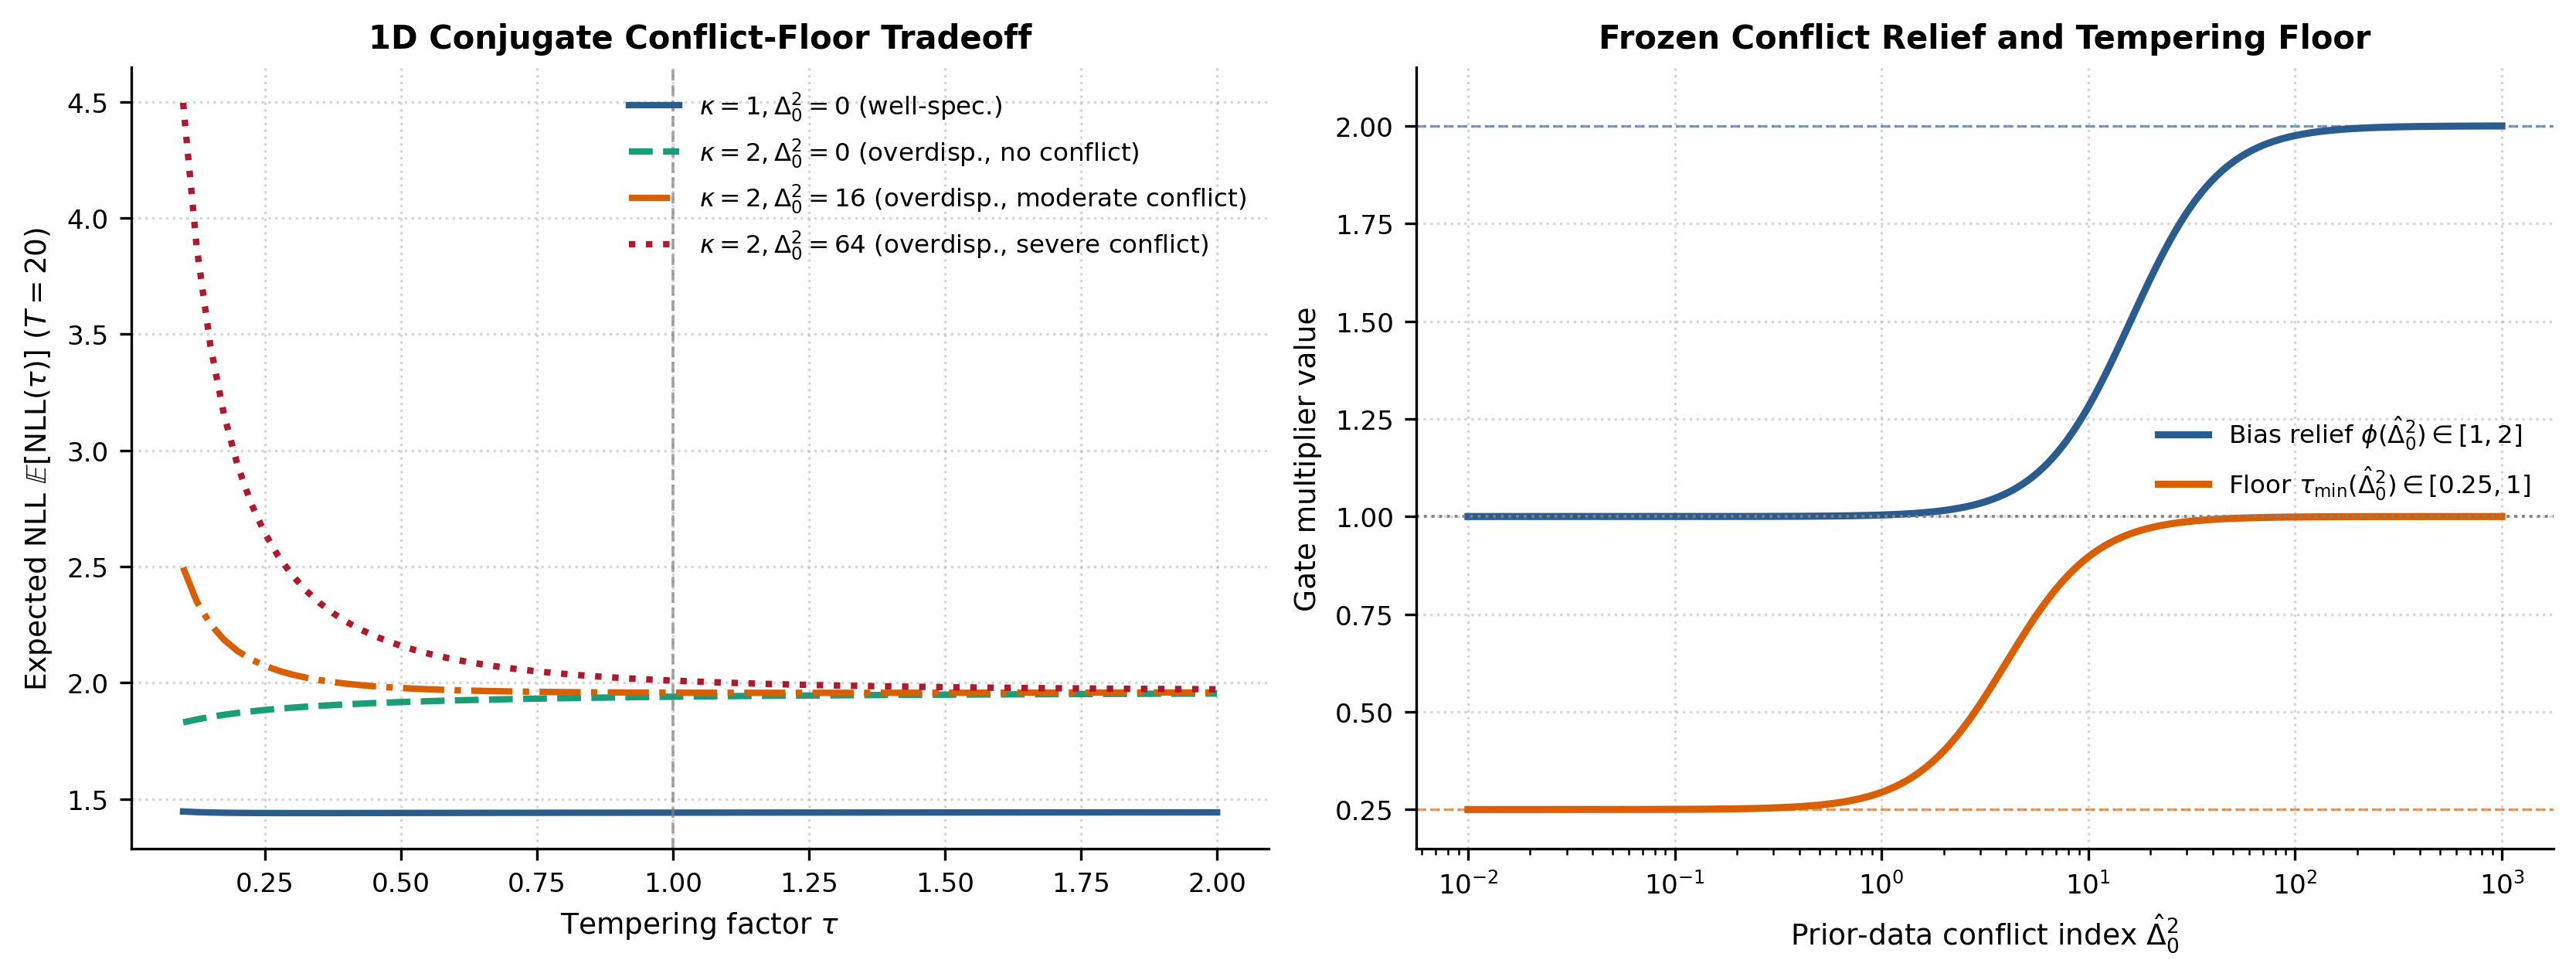
\includegraphics[width=0.98\textwidth]{figures/fig2_conflict_floor_nll.png}
\caption{Left: 1D conjugate expected NLL at $T=20$ from \cref{thm:conflict_floor}, showing optimal tempering shifting from $\tau < 1$ under pure overdispersion ($\kappa=2, \Delta_0^2=0$, optimum $\tau = 0.10$) to $\tau > 1$ under severe prior conflict ($\kappa=2, \Delta_0^2=64$, optimum $\tau = 2.00$). Right: frozen online conflict multiplier $\phi(\hat{\Delta}_0^2) \in [1, 2]$ and tempering floor $\tau_{\min}(\hat{\Delta}_0^2) \in [0.25, 1]$.}\label{fig:conflict_floor}
\end{figure}

\begin{theorem}[Conjugate NLL vs.\ Sample-Pair MSE Tradeoff]\label{thm:conflict_floor}
In a 1D conjugate Gaussian location model $Y_1, \dots, Y_T \stackrel{\mathrm{i.i.d.}}{\sim} \Ncal(\theta^*, \kappa\sigma^2)$ ($\kappa > 0$) with prior $\theta \sim \Ncal(\mu_0, \sigma_0^2)$, define prior-variance ratio $r_0 = \sigma^2 / \sigma_0^2 > 0$, standardized prior conflict $\Delta_0^2 = (\theta^* - \mu_0)^2 / \sigma_0^2 \ge 0$, and inverse-precision coordinate $u(\tau) = (r_0 + \tau T)^{-1}$. Under Gibbs updating $\pi_\tau(\theta \mid Y_{1:T}) = \Ncal(\mu_{\mathrm{post},\tau}, \sigma_{\mathrm{post},\tau}^2)$ with $\sigma_{\mathrm{post},\tau}^2 = u(\tau)\sigma^2$, predicting independent test draw $Y_{\mathrm{true}} \sim \Ncal(\theta^*, \kappa\sigma^2)$ with posterior-predictive draw $Y_{\mathrm{pred}} \sim \Ncal(\mu_{\mathrm{post},\tau}, \sigma^2 + \sigma_{\mathrm{post},\tau}^2)$ yields exact expectations in $u = u(\tau)$:
\begin{align}
\E\bigl[\mathrm{NLL}(u)\bigr] &= \frac{1}{2}\log(2\pi\sigma^2) + \frac{1}{2}\log(1 + u) + \frac{\kappa + r_0 \Delta_0^2 u^2 + (1 - r_0 u)^2 \kappa / T}{2(1 + u)}, \label{eq:exact_nll_1d}\\
\E\bigl[(Y_{\mathrm{pred}} - Y_{\mathrm{true}})^2\bigr] &= \sigma^2\Bigl(1 + u + \kappa + r_0 \Delta_0^2 u^2 + \frac{(1 - r_0 u)^2 \kappa}{T}\Bigr). \label{eq:exact_mse_1d}
\end{align}
Evaluating initial $u$-derivatives at $u = 0$ (decreasing $\tau$ increases $u$) gives
\begin{align*}
\left.\frac{\partial \E[\mathrm{NLL}(u)]}{\partial u}\right|_{u=0} &= \frac{1 - \kappa}{2} - \frac{\kappa(1 + 2 r_0)}{2 T}, &
\left.\frac{\partial \E[(Y_{\mathrm{pred}} - Y_{\mathrm{true}})^2]}{\partial u}\right|_{u=0} &= \sigma^2\Bigl(1 - \frac{2 r_0 \kappa}{T}\Bigr).
\end{align*}
Consequently, under variance overdispersion ($\kappa > 1$) whenever $T > 2 r_0 \kappa$, decreasing $\tau$ reduces expected predictive NLL ($\partial_u \E[\mathrm{NLL}]|_{u=0} < 0$) while simultaneously increasing expected sample-pair MSE ($\partial_u \E[\mathrm{MSE}_{\mathrm{pred}}]|_{u=0} > 0$), whereas large prior conflict $\Delta_0^2$ generates an $\mathcal{O}(\Delta_0^2 u^2)$ NLL penalty (\cref{fig:conflict_floor}) requiring $\tau$ relief.
\end{theorem}

Finite-difference derivative verification across all 20 pairs $(\kappa, T) \in \{1.0, 1.5, 2.0, 4.0, 6.25\} \times \{20, 50, 200, 1000\}$ agrees with \cref{thm:conflict_floor} to max error $3.19 \times 10^{-9}$ (NLL) and $6.58 \times 10^{-9}$ (MSE). Notably, for our Benchmark 3 error-distribution parameters ($T=20, r_0=1, \kappa=(1.0/0.4)^2=6.25$), \cref{thm:conflict_floor} predicts $\partial_u \E[\mathrm{MSE}_{\mathrm{pred}}/\sigma^2]|_{u=0} = 1 - 12.5/20 = +0.375 > 0$, directly explaining why tempering lowers NLL and MMD while slightly elevating sample-pair RMSE.

\subsection{Dispersion gating, contamination bounds, and asymptotic calibration}

\begin{proposition}[Finite-Sample Chi-Squared Dispersion Bound]\label{prop:chi2_domination}
Suppose conditional on fixed (non-adaptive) designs $\xi_{1:t}$ the true simulator satisfies $Y_j \mid \xi_j \sim \Ncal(\mu_{\theta^*}(\xi_j), \sigma^2)$ independently, the model mean is linear $\mu_\theta(\xi_j) = \phi_j^\top \theta$ with full column rank design matrix $\Phi_{1:t} \in \R^{t \times p}$ ($\mathrm{rank}(\Phi_{1:t}) = p$ for $t \ge p$), and $\hat{\sigma}_{\mathrm{ep},j}^2 = \phi_j^\top \hat{\Sigma}_t \phi_j \ge 0$ for any (possibly random) symmetric positive semidefinite covariance $\hat{\Sigma}_t \succeq 0$. For the unbiased ordinary least-squares estimator $\hat{\theta}_{\mathrm{OLS}} = (\Phi_{1:t}^\top \Phi_{1:t})^{-1} \Phi_{1:t}^\top Y_{1:t}$, the standardized predictive dispersion statistic $S_t^{\mathrm{pred}} = \sum_{j=1}^t (Y_j - \phi_j^\top \hat{\theta}_{\mathrm{OLS}})^2 / (\sigma^2 + \hat{\sigma}_{\mathrm{ep},j}^2)$ is stochastically dominated by $\chi^2_{t-p}$ and hence by $\chi^2_t$ in finite samples: for all $x \ge 0$, $\Prob(S_t^{\mathrm{pred}} > x \mid \xi_{1:t}) \le \Prob(\chi^2_{t-p} > x) \le \Prob(\chi^2_t > x)$. Under prior shrinkage $\hat{\theta}_t - \hat{\theta}_{\mathrm{OLS}} = \mathcal{O}_p(\Delta_0 t^{-1})$ ($\Delta_0 = \|P_0^{1/2}(\theta^* - \mu_0)\|_2$) with uniformly bounded $\|\phi_j\|_2 \le L_\mu$ and $\max_{1\le j\le t}\hat{\sigma}_{\mathrm{ep},j}^2 = \mathcal{O}_p(t^{-1})$, exact OLS residual orthogonality $(Y_{1:t} - \Phi_{1:t}\hat{\theta}_{\mathrm{OLS}})^\top \Phi_{1:t} = 0$ eliminates the leading $\sigma^{-2}$ cross-term identically, leaving an unnormalized excess $\mathcal{O}_p((\Delta_0^2 + \Delta_0)/t)$ controlled online by $\tau_{\min}(\hat{\Delta}_0^2)$.
\end{proposition}

\begin{assumption}[Regularity for Unified GatedC G-LHW Guarantees]\label{assump:regularity}
Assume: (A1) $\sigma_\theta(\xi) \equiv \sigma > 0$ on compact parameter domain $\Theta \subset \R^p$ containing $\theta^*$ in its interior; (A2) $\theta \mapsto \mu_\theta(\xi)$ is $C^2$ over $\Theta \times \Xcal$ with uniform bounds $|\mu_\theta(\xi)| \le M_\mu$, $\|\nabla_\theta \mu_\theta(\xi)\|_2 \le L_\mu$, and $\|\nabla_\theta^2 \mu_\theta(\xi)\|_{\mathrm{op}} \le K_\mu$ and equicontinuous Hessian $\theta \mapsto \nabla_\theta^2 \mu_\theta(\xi)$ at $\theta^*$ uniformly over $\Xcal$, empirical design information $\bar{G}_t = t^{-1}\sum_{j=1}^t \nabla_\theta \mu_{\theta^*}(\xi_j)\nabla_\theta \mu_{\theta^*}(\xi_j)^\top \succeq \lambda_{\min} I_p \succ 0$ holds for $t \ge t_0$, and predictable ($\mathcal{F}_{j-1}$-measurable) sequential designs $\xi_j$ satisfy Wald mean identifiability: for every $\delta > 0$, $\liminf_{t\to\infty} \inf_{\|\theta - \theta^*\|_2 \ge \delta} t^{-1}\sum_{j=1}^t (\mu_\theta(\xi_j) - \mu_{\theta^*}(\xi_j))^2 > 0$ in probability; (A3) empirical centerings satisfy $\max_{1\le j \le t} |\hat{\mu}_{t,j} - \mu_{\theta^*}(\xi_j)| \to_p 0$ and the diagnostic statistics admit limits $S_t^{\mathrm{pred}} / t \to_p s_\infty \in (0, \infty)$ and $\hat{\Delta}_0^2 \to_p \Delta_{0,\infty}^2 \in [0, \infty)$; (A4) in the contaminated regime $Y_j \mid \xi_j \sim (1 - \varepsilon)\Ncal(\mu_{\theta^*}(\xi_j), \sigma^2) + \varepsilon Q_{\mathrm{out}, j}$ ($\varepsilon \in [0, 1)$), $Q_{\mathrm{out}, j}$ is symmetric around $\mu_{\theta^*}(\xi_j)$ (arbitrary heavy tails permitted, requiring no finite moments) with uniform bulk tightness $\inf_j P^*(|Y_j - \mu_{\theta^*}(\xi_j)| \le R_0 \mid \xi_j) \ge \eta_0 > 0$ for some $R_0 < \infty$ and $\eta_0 > 0$.
\end{assumption}

\begin{theorem}[Rate Envelope, Huber Outlier Bound, Consistency, and Godambe Calibration]\label{thm:gatedc_guarantees}
Let $(\omega_t, c_t)$ follow the frozen GatedC G-LHW gate (\cref{sec:algorithm}) with $p_{\mathrm{IMQ}} = 1$.
\begin{enumerate}[label=(\alph*)]
\item \textbf{Unconditional rate envelope.} For all $t \ge 1$, $\hat{\Delta}_0^2 \ge 0$, and $S_t^{\mathrm{pred}} \ge 0$,
\[
0.25\,\omega_0(5\sigma) \le \omega_t \le 2.0\,\omega_0(2\sigma),
\]
equivalently $\omega_t \in [0.128766574328\sigma^2,\, 1.061024534381\sigma^2]$.
\item \textbf{Bounded Huber gross-error sensitivity and outlier shift.} Under (A1)--(A2), for any centering $\hat{\mu}_j$ with bounded $|\mu_\theta(\xi_j) - \hat{\mu}_j| \le 2M_\mu$, the PredC score gradient $\nabla_\theta \ell_B(\theta; y_j, \xi_j; \hat{\mu}_j, c_t)$ remains uniformly bounded for all $y_j \in \R$, with Euclidean norm at $\mu_\theta(\xi_j) = \hat{\mu}_j$ equal to $\frac{2}{\sigma^3}|\psi_B(z; c_t/\sigma, 1)|\,\|\nabla_\theta \mu_\theta(\xi_j)\|_2 \le \frac{2 L_\mu}{\sigma^3}\sup_z|\psi_B(z; 5, 1)| = \frac{2 L_\mu}{\sigma^3}(2.6019195361\dots)$. In the linear conjugate model (\cref{sec:algorithm}) with $P_0 \succ 0$ and bounded $\hat{\mu}_j$ (or under annealed continuation whenever strictly fewer than half of observations are corrupted, in particular $t \ge 3$ under single-point corruption), moving any single observation $|y_1| \to \infty$ produces a uniformly bounded change $\|\hat{\theta}_{\mathrm{post}}(y_1, y_{2:t}) - \hat{\theta}_{\mathrm{post}}^{\mathrm{clean}}\|_2 \le C_{\mathrm{out}} < \infty$~\cite{huber1964robust}, whereas standard BOED diverges linearly as $\Theta(|y_1|)$.
\item \textbf{M-estimator consistency.} Under (A1)--(A4), any empirical risk minimizer $\hat{\theta}_t^{\mathrm{GBOED}} \in \arg\min_{\theta \in \Theta} \sum_{j=1}^t \ell_B(\theta; Y_j, \xi_j; \hat{\mu}_{t,j}, c_t)$ satisfies $\hat{\theta}_t^{\mathrm{GBOED}} \to_p \theta^*$ as $t \to \infty$ under both well-specified Gaussian sampling ($\varepsilon = 0$) and symmetric heavy-tailed $\varepsilon$-contamination ($\varepsilon \in [0, 1)$).
\item \textbf{Asymptotic Godambe covariance.} Under (A1)--(A3) and $\varepsilon = 0$, the asymptotic Gibbs posterior covariance satisfies
\[
\Sigma_{\mathrm{Gibbs}, T} = \frac{1}{T \gamma_\infty}\,\bar{H}_T(c_T)^{-1}\bar{J}_T(c_T)\bar{H}_T(c_T)^{-1}\bigl(1 + o_p(1)\bigr), \qquad
\gamma_\infty = \phi(\Delta_{0,\infty}^2)\,\tau_\infty \in [0.25,\, 2.0],
\]
where $c_T \in \{2\sigma, 5\sigma\}$ is the active threshold branch and $\tau_\infty = 1$ whenever $s_\infty \le 1$. When $\Delta_{0,\infty}^2 = 0$ and $s_\infty \le 1$, $\gamma_\infty = 1$ yields exact asymptotically calibrated frequentist sandwich coverage on both threshold branches; when prior conflict persists ($\Delta_{0,\infty}^2 > 0$, up to $\phi \to 2$), the fixed-prior rule trades mild variance tightening ($\gamma_\infty \in (1, 2]$) to halve finite-sample prior-trap bias before asymptotic shrinkage completes.
\end{enumerate}
\end{theorem}

The Huber outlier saturation audit (\texttt{results/audit\_results.json}) illustrates \cref{thm:gatedc_guarantees}(b) numerically on a 12-point linear design ($\beta^* = (10, -7)^\top, \sigma = 0.5$): corrupting $y_1$ across $10, 10^2, 10^4, 10^6$ drives standard BOED posterior norm from $9.31$ up to $97{,}179.69$, whereas AnnealedPredC GatedC keeps posterior parameter norm within $[12.0704, 12.0718]$ and error vs.\ clean fit within $[0.1464, 0.1483]$ (saturating at $12.0717$ and $0.1467$ for $y_1 \ge 10^4$).

\section{The Frozen GatedC G-LHW Rule, Continuation, and Baseline Audit}\label{sec:algorithm}

To prevent data-snooping or hidden scenario tuning, \cref{tab:hyperparams} separates analytical quantities determined purely by LHW theory and quadrature (\cref{prop:stein_fisher,cor:multivariate_lhw}) from frozen engineering gate constants held identical across every benchmark, scenario, noise level, and dimension.

\begin{table}[t]
\centering
\small
\caption{Strict separation of analytically derived LHW constants and frozen algorithm hyperparameters across all experiments.}\label{tab:hyperparams}
\begin{tabular}{@{}lll@{}}
\toprule
Quantity & Origin & Exact value / rule \\
\midrule
$\omega_0(2\sigma)/\sigma^2$, $\omega_0(5\sigma)/\sigma^2$ & Analytic + 50-digit \texttt{arb} & $0.5305122672$, $0.5150662973$ \\
$H_B^2/J_B$ (Godambe eff.) & Analytic (\cref{prop:stein_fisher}) & $0.8942$ ($r=2$), $0.9931$ ($r=5$) \\
Variance floor bounds $[0.25, 1.0]$ & Rate envelope & $0.25\,\omega_0(5\sigma)$ to $1.0\,\omega_0(c_t)$ \\
Warmup horizon & Parameter count $p$ & $t < p + 2$ fixes $\tau_t = 1$, $c_t = 2\sigma$ \\
$\chi^2$ gate quantiles & Frozen engineering choice & $\chi^2_{t, 0.85}$ (threshold), $\chi^2_{t, 0.95}$ (tempering) \\
Conflict relief $\phi(\hat{\Delta}_0^2)$ & Frozen smooth gate & $1 + \hat{\Delta}_0^4 / (\hat{\Delta}_0^4 + 16^2) \in [1, 2]$ \\
Tempering floor $\tau_{\min}(\hat{\Delta}_0^2)$ & Frozen smooth gate & $1 - 0.75 / (1 + (\hat{\Delta}_0^2 / 4)^2) \in [0.25, 1]$ \\
AnnealedPredC $\lambda$-ladder & Frozen pure-Bayes schedule & $(1.0,\, 0.5,\, 0.25,\, 0.1,\, 0.0)$ from $\mu_0(\xi)$ \\
\bottomrule
\end{tabular}
\end{table}

\subsection{Frozen design-time and online GatedC G-LHW equations}
At design time, prior samples $\Theta_0$ and design points $\Xcal_0$ are passed with $p_{\mathrm{IMQ}} > 1/2$ (fixed at $p_{\mathrm{IMQ}} = 1$) to compute $\rho_\theta$ and $\rho_\xi$ (\cref{def:variations}). Provided $\rho_\theta \le 10^{-6}$ and $\rho_\xi \le 10^{-6}$, the calibrated baseline rates $\omega_0(2\sigma)$ and $\omega_0(5\sigma)$ are cached once from \cref{tab:quadrature}. Online at step $t \ge 1$, given pilot posterior draws $q_{t,\mathrm{pil}}$, we compute empirical prior-data conflict $\hat{\Delta}_0^2 = (1/p)\E_{q_{t,\mathrm{pil}}}[(\theta - \mu_0)^\top \Sigma_0^{-1} (\theta - \mu_0)]$ and standardized dispersion $S_t^{\mathrm{pred}} = \sum_{j=1}^t (y_j - \hat{\mu}_{t,\mathrm{pil}}(\xi_j))^2 / (\sigma^2 + \hat{\sigma}_{\mathrm{ep}, t, j}^2)$. Specifically, in conjugate linear regression (\nolinkurl{scripts/run_regression_benchmark.py}), $q_{t,\mathrm{pil}}$ is formed via an online two-stage pilot: five-step AnnealedPredC at $(2\sigma, \omega_0(2\sigma))$ yields initial conflict $\hat{\Delta}_{0,\mathrm{init}}^2$, and a second five-step AnnealedPredC fit at $(2\sigma, \omega_0(2\sigma)\phi(\hat{\Delta}_{0,\mathrm{init}}^2))$ supplies $(q_{t,\mathrm{pil}}, \hat{\Delta}_0^2, S_t^{\mathrm{pred}})$ before evaluating the gated target $(\omega_t, c_t)$. In the GPU nonlinear SMC suites (\nolinkurl{scripts/_smc_gpu.py}), $q_{t-1}$ provides predictive centers $\hat{\mu}_j = \E_{q_{t-1}}[\mu_\theta(\xi_j)]$ and a one-step importance-reweighted pilot $q_{t,\mathrm{pil}}$ using the previous conflict factor $\phi_{t-1}$ before resampling and Metropolis--Hastings updates at $(\omega_t, c_t)$ without multi-step scale annealing. Then:
\[
\phi(\hat{\Delta}_0^2) = 1 + \frac{\hat{\Delta}_0^4}{\hat{\Delta}_0^4 + 16^2}, \qquad
\tau_{\min}(\hat{\Delta}_0^2) = 1 - \frac{0.75}{1 + (\hat{\Delta}_0^2 / 4)^2},
\]
and for $t < p + 2$, $(c_t, \omega_{0,t}, \tau_t) = (2\sigma, \omega_0(2\sigma), 1)$, whereas for $t \ge p + 2$,
\begin{align*}
\tau_t &= \begin{cases} 1, & S_t^{\mathrm{pred}} \le \chi^2_{t, 0.95}, \\ \max\!\bigl(\tau_{\min}(\hat{\Delta}_0^2),\, t / S_t^{\mathrm{pred}}\bigr), & S_t^{\mathrm{pred}} > \chi^2_{t, 0.95}, \end{cases}\\
(c_t, \omega_{0,t}) &= \begin{cases} (5\sigma, \omega_0(5\sigma)), & S_t^{\mathrm{pred}} \le \chi^2_{t, 0.85}, \\ (2\sigma, \omega_0(2\sigma)), & S_t^{\mathrm{pred}} > \chi^2_{t, 0.85}, \end{cases}
\end{align*}
setting final $\omega_t = \omega_{0,t}\,\phi(\hat{\Delta}_0^2)\,\tau_t$. Intuitively, under severe prior conflict ($\hat{\Delta}_0^2 \gg 16$), $\phi \to 2$ doubles the rate to clear the prior trap and $\tau_{\min} \to 1$ protects against conflict-induced tempering; under genuine overdispersion ($\hat{\Delta}_0^2$ small, $S_t^{\mathrm{pred}} > \chi^2_{t, 0.95}$), $\tau_t$ drops toward $0.25$ and $c_t$ tightens to $2\sigma$.

\subsection{Pure-Bayesian AnnealedPredC conjugate continuation}
To prevent single-pass PredC weight collapse (\cref{prop:prior_trap}(b)) without resorting to non-Bayesian regression heuristics (such as Theil--Sen or RANSAC), we initialize predictive centering strictly from the Bayesian prior mean $\hat{\mu}^{(0)} = \Phi \mu_0$, set $c_{\max} = \max(2\sigma,\, \mathrm{med}_j |y_j - \hat{\mu}^{(0)}_j| + 2\sigma)$, and sweep scales $c^{(s)} = 2\sigma + \lambda_s(c_{\max} - 2\sigma)$ along $\lambda_s \in (1.0, 0.5, 0.25, 0.1, 0.0)$, updating the exact closed-form PredC Gaussian posterior at each step (\cref{prop:conjugate_predc}) before evaluating the gated target $(c_t, \omega_t)$.

\begin{proposition}[Exact Conjugate PredC IMQ-WSM Normal Equations~\cite{altamirano2024rcgp}]\label{prop:conjugate_predc}
For a linear model $\mu_\theta(\xi_j) = \phi_j^\top \theta$ with prior $\Ncal(\mu_0, P_0^{-1})$, fixed predictive centers $\hat{\mu}_j \in \R$, threshold $c > 0$, and learning rate $\omega > 0$, the PredC IMQ-WSM generalized posterior $\pi^{\omega}(\theta) \propto \exp\bigl(-\frac{1}{2}\|\theta - \mu_0\|_{P_0}^2 - \omega \sum_{j=1}^t \ell_B(\phi_j^\top\theta; y_j, \hat{\mu}_j, c)\bigr)$ is exact multivariate Gaussian $\Ncal(m_{\mathrm{post}}, P_{\mathrm{post}}^{-1})$ with
\[
P_{\mathrm{post}} = P_0 + \frac{2\omega}{\sigma^4}\sum_{j=1}^t m_j^2\,\phi_j \phi_j^\top, \qquad
P_{\mathrm{post}}\,m_{\mathrm{post}} = P_0 \mu_0 + \frac{2\omega}{\sigma^4}\sum_{j=1}^t \bigl(m_j^2 y_j - \sigma^2 (m^2)'_j\bigr)\phi_j,
\]
where $m_j^2 = m(y_j; \hat{\mu}_j, c)^2$ and $(m^2)'_j = \partial_y [m(y_j; \hat{\mu}_j, c)^2]$.
\end{proposition}

BFGS numerical minimization of the raw objective \eqref{eq:predc_loss_def} matches \cref{prop:conjugate_predc} to $3.486 \times 10^{-8}$ parameter $L_2$-difference and $1.132 \times 10^{-11}$ central finite-difference gradient norm.

\subsection{Forensic audit of the anchor implementation}\label{sec:barlas_audit}
Inspection of the public reference repository (\nolinkurl{yasirbarlas/GBOED}, commit \texttt{c2b9c63}) shows two contrasting facts verified in \nolinkurl{scripts/verify_theorem_and_barlas_audit.py} (\nolinkurl{results/audit_results.json}):
\begin{enumerate}[label=(\arabic*)]
\item \emph{PredC implementation confirmed:} The loss classes in \nolinkurl{utils/loss_functions.py} (lines 83, 144, and 222 across regression, location finding, and pharmacokinetics) compute the predictive mean $\hat{\mu} = \mathrm{mean}(\mu_\theta)$ and centered differences directly, matching~\eqref{eq:predc_loss_def}.
\item \emph{Effective learning-rate cubic scaling ($w^3$):} Inside \nolinkurl{utils/loss_functions.py} (lines 90, 92, 150--151, 228--229), the weighted loss multiplies by \nolinkurl{self.w**2} within \nolinkurl{dm_weighted}, and the task scripts (\nolinkurl{regression.py:340}, \nolinkurl{location.py:406}, \nolinkurl{pharmacokinetic.py:419}, and \nolinkurl{utils/gibbs_eig.py:59,92}) multiply the returned potential by $-w$ again, yielding an effective learning rate $w^3$. For nominal $w = 0.4$ ($w = 0.2$), this produces $w^3 = 0.064$ ($w^3 = 0.008$), attenuating updates to $16\%$ ($4\%$) of intended nominal strength. All baseline evaluations in \cref{sec:benchmarks} remove this duplicate multiplication so comparisons evaluate intended schedules fairly.
\end{enumerate}

\section{Sequential Experimental Design Benchmarks and Ablations}\label{sec:benchmarks}

We benchmark the single frozen GatedC G-LHW rule via \nolinkurl{scripts/run_all_benchmarks.py} across three sequential experimental design suites matching the protocols and Appendix metrics (RMSE, kernel MMD$^2$ via median heuristic bandwidth, and predictive NLL over 500 holdout designs in Suites 1 and 3 and 100 equispaced points on $[-4, 4]$ in Suite 2, with 1000 evaluation draws per replicate) of Barlas et al.~\cite{barlas2025gboed} on an NVIDIA GeForce RTX 4070 CUDA GPU:
\begin{enumerate}[label=\arabic*.]
\item \textbf{Location Finding ($d=4, K=2, p=8, T=30, R=90, M=1024$):} Two sources with $\theta^* \sim \Ncal(0, I_8)$ per replicate, intensity $\log(0.1 + \sum_{k=1}^2 (\|\theta_k - \xi\|_2^2 + 10^{-4})^{-1})$, simulator $\sigma = 0.5$, Gibbs NMC EIG acquisition ($256 \times 256$) over $384$ uniform and posterior-guided candidates per step; scenarios: well-specified (\texttt{none}), $30\%$ negative uniform outliers $3\sigma$--$7\sigma$ (\texttt{outlier}), and overdispersed Gaussian noise $\sigma_{\mathrm{true}} = 0.8$ (\texttt{error-dist}). Baseline \texttt{Barlas\_ExpDecay} uses Barlas's published nonlinear schedule $c_t = 1.8 e^{-0.06(t-1)} + 0.2, \omega = 0.4$.
\item \textbf{Bayesian Linear Regression ($p=2, T=10, R=270$):} Equal splits across true parameter/noise pairs $(10,-7), \sigma=1.2$; $(-3,8), \sigma=0.8$; and $(9,9), \sigma=1.0$ under strongly conflicted prior $\Ncal(0, I_2)$ on $\xi \in [-4, 4]$ ($100$ equispaced holdout designs matching Barlas et al.); scenarios: \texttt{none} (prior conflict), \texttt{outlier} ($30\%$ negative shifts $3\sigma$--$9\sigma$), and true \texttt{laplace} error draws with scale $\sigma$, evaluated with Gibbs NMC EIG and AnnealedPredC posterior updates across seven methods and ablations (comparing transferred \texttt{Barlas\_Transf.} with $c_t = 1.8 e^{-0.06(t-1)} + 0.2, \omega = 0.4$ against regression-tuned \texttt{Barlas\_Regr.} with $c_t = 9.0 e^{-0.3(t-1)} + 1.0, \omega = 0.4$).
\item \textbf{Nonlinear Radial-Sinusoidal Design ($p=3, T=20, R=90, M=1024$):} Well-specified prior $\theta^* \sim \Ncal(0, I_3)$, $\mu_\theta(\xi) = 2\exp(-\|\xi - \theta_{1:2}\|_2^2 / 2.88) + \theta_3\sin(0.8(\xi_1+\xi_2))$, $\sigma = 0.4$, $\xi \in [-3,3]^2$, scenarios: \texttt{none}, $30\%$ outliers (\texttt{outlier}), and severe overdispersion $\sigma_{\mathrm{true}} = 1.0$ (\texttt{error-dist}, $\kappa = 6.25$).
\end{enumerate}

\begin{figure}[t]
\centering
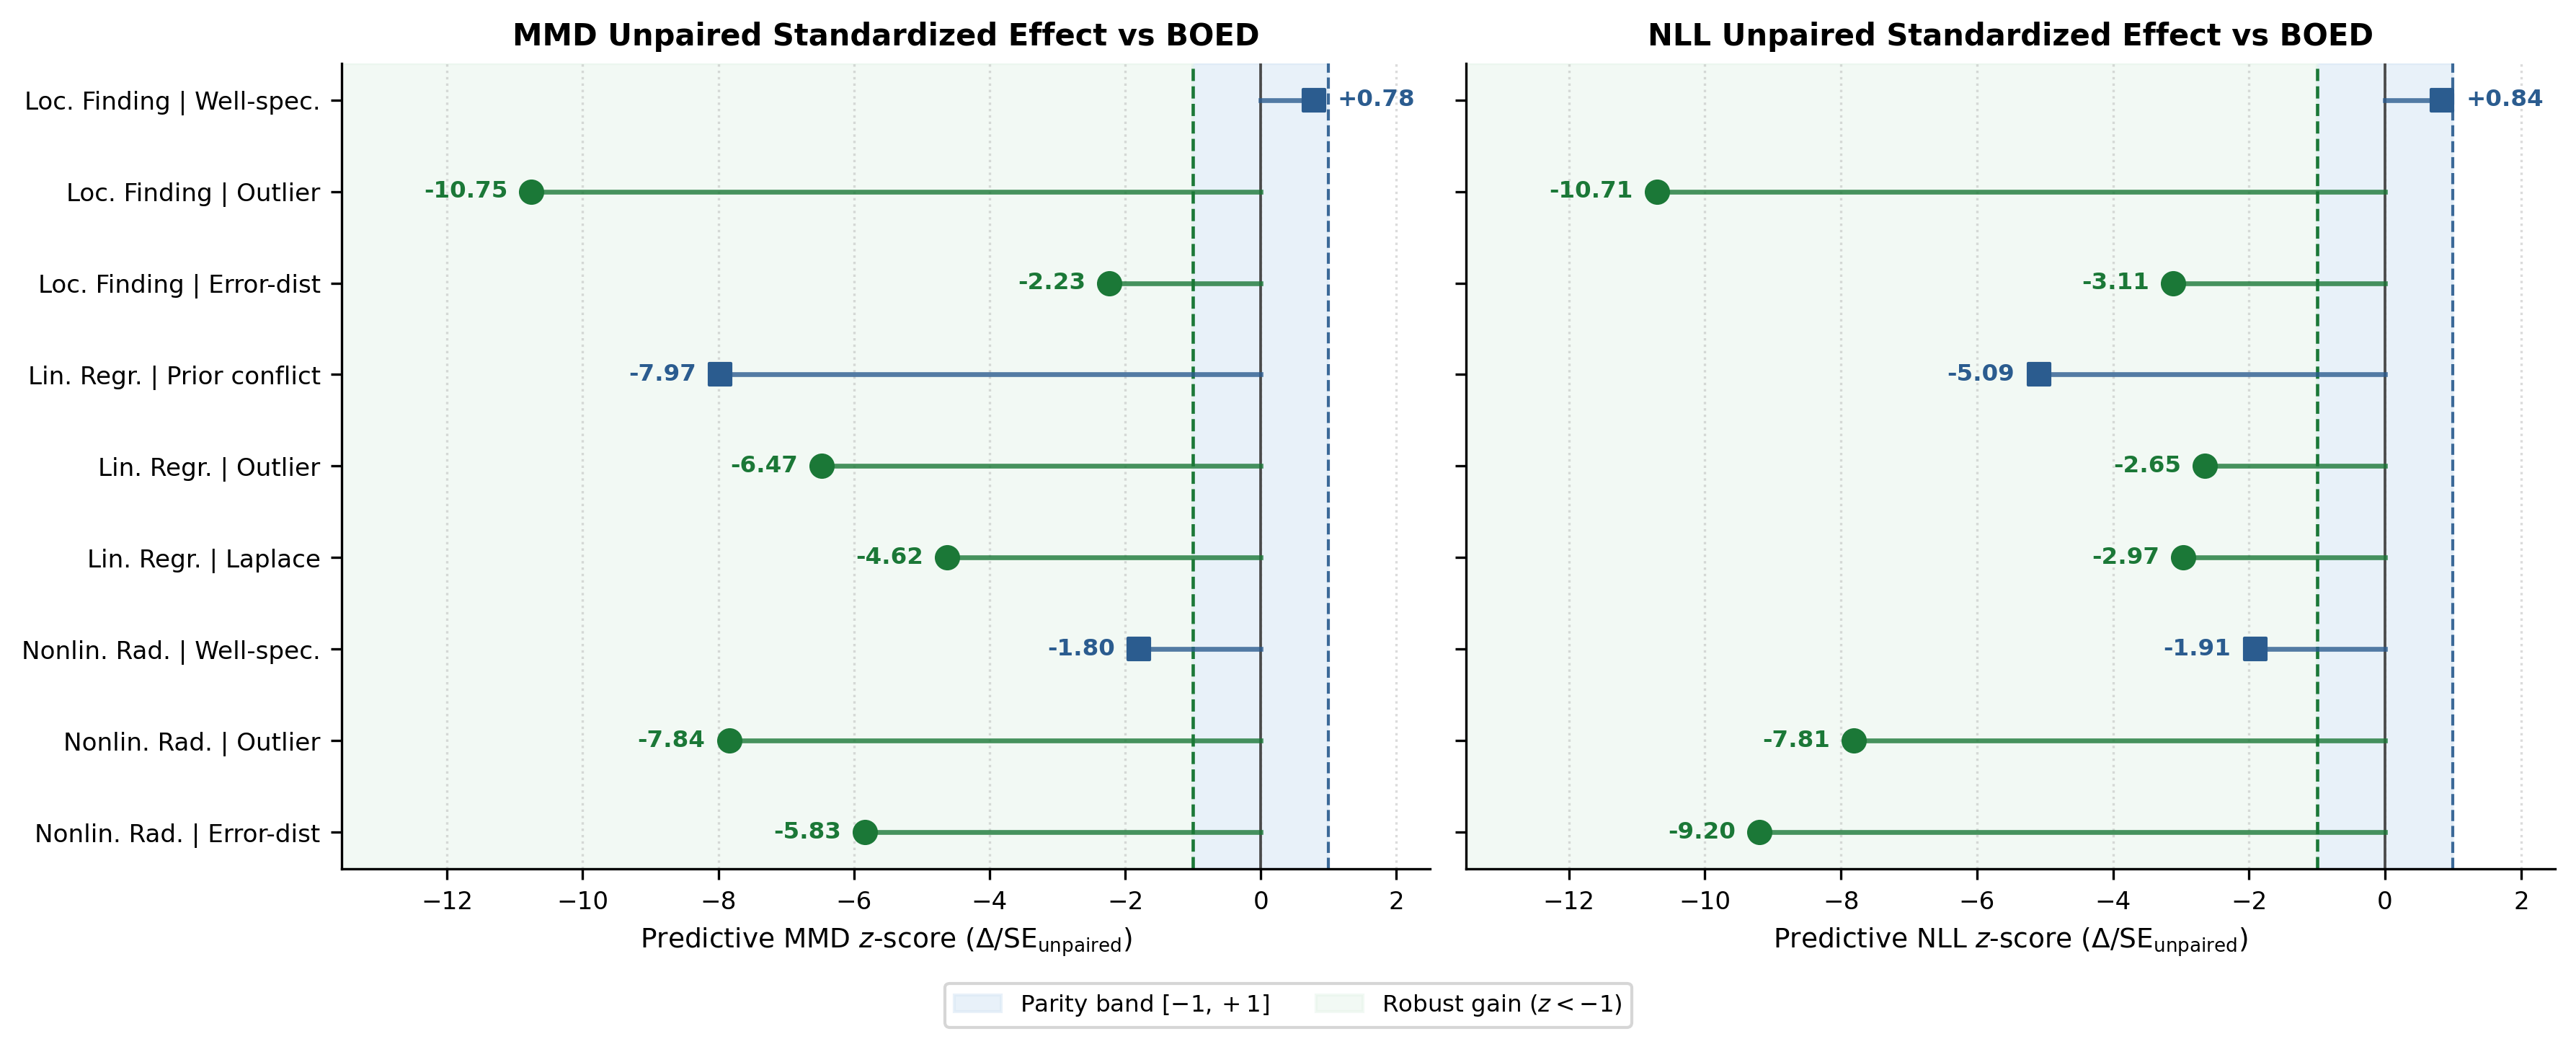
\includegraphics[width=0.98\textwidth]{figures/fig1_benchmark_forest.png}
\caption{Unpaired standardized effects $z_{\mathrm{uSE}} = (\bar{M}_{\mathrm{GatedC}} - \bar{M}_{\mathrm{BOED}}) / (\mathrm{SE}_{\mathrm{GatedC}}^2 + \mathrm{SE}_{\mathrm{BOED}}^2)^{1/2}$ across all nine benchmark-scenario pairs ($R=90$ or $270$). Every well-specified scenario satisfies $z_{\mathrm{uSE}} \le +0.84$ on both MMD and NLL, while all six misspecified scenarios improve significantly with $z_{\mathrm{uSE}} \in [-10.75, -2.23]$.}\label{fig:forest}
\end{figure}

\begin{table}[t]
\centering
\scriptsize
\setlength{\tabcolsep}{3pt}
\caption{Cross-benchmark comparison of standard BOED against the single frozen GatedC G-LHW rule (means $\pm$ SE stacked below; unpaired standardized effect $z_{\mathrm{uSE}}$, negative favors GatedC).}\label{tab:main_results}
\begin{tabular}{@{}lccccccccc@{}}
\toprule
Scenario & \multicolumn{3}{c}{Standard BOED} & \multicolumn{3}{c}{Frozen GatedC G-LHW} & \multicolumn{3}{c}{$z_{\mathrm{uSE}}$ (GatedC vs.\ BOED)} \\
\cmidrule(lr){2-4}\cmidrule(lr){5-7}\cmidrule(lr){8-10}
& RMSE & MMD & NLL & RMSE & MMD & NLL & RMSE & MMD & NLL \\
\midrule
\multicolumn{10}{@{}l}{\textbf{Location Finding ($d=4, K=2, p=8, T=30, R=90$)}} \\
\texttt{none} & \begin{tabular}{@{}c@{}}$0.7276$\\[-2pt]{\tiny$\pm0.0015$}\end{tabular} & \begin{tabular}{@{}c@{}}$0.0106$\\[-2pt]{\tiny$\pm0.0009$}\end{tabular} & \begin{tabular}{@{}c@{}}$0.7573$\\[-2pt]{\tiny$\pm0.0028$}\end{tabular} & \begin{tabular}{@{}c@{}}$0.7291$\\[-2pt]{\tiny$\pm0.0016$}\end{tabular} & \begin{tabular}{@{}c@{}}$0.0116$\\[-2pt]{\tiny$\pm0.0010$}\end{tabular} & \begin{tabular}{@{}c@{}}$0.7608$\\[-2pt]{\tiny$\pm0.0031$}\end{tabular} & $+0.71$ & $+0.78$ & $+0.84$ \\
\texttt{outlier} & \begin{tabular}{@{}c@{}}$0.7897$\\[-2pt]{\tiny$\pm0.0036$}\end{tabular} & \begin{tabular}{@{}c@{}}$0.0498$\\[-2pt]{\tiny$\pm0.0027$}\end{tabular} & \begin{tabular}{@{}c@{}}$0.8837$\\[-2pt]{\tiny$\pm0.0091$}\end{tabular} & \begin{tabular}{@{}c@{}}$0.7509$\\[-2pt]{\tiny$\pm0.0020$}\end{tabular} & \begin{tabular}{@{}c@{}}$0.0189$\\[-2pt]{\tiny$\pm0.0010$}\end{tabular} & \begin{tabular}{@{}c@{}}$0.7808$\\[-2pt]{\tiny$\pm0.0031$}\end{tabular} & $-9.51$ & $-10.75$ & $-10.71$ \\
\texttt{error-dist} & \begin{tabular}{@{}c@{}}$0.9657$\\[-2pt]{\tiny$\pm0.0013$}\end{tabular} & \begin{tabular}{@{}c@{}}$0.0501$\\[-2pt]{\tiny$\pm0.0005$}\end{tabular} & \begin{tabular}{@{}c@{}}$1.5131$\\[-2pt]{\tiny$\pm0.0031$}\end{tabular} & \begin{tabular}{@{}c@{}}$0.9671$\\[-2pt]{\tiny$\pm0.0012$}\end{tabular} & \begin{tabular}{@{}c@{}}$0.0486$\\[-2pt]{\tiny$\pm0.0005$}\end{tabular} & \begin{tabular}{@{}c@{}}$1.4994$\\[-2pt]{\tiny$\pm0.0031$}\end{tabular} & $+0.80$ & $-2.23$ & $-3.11$ \\
\midrule
\multicolumn{10}{@{}l}{\textbf{Bayesian Linear Regression ($p=2, T=10, R=270$, conflicted prior)}} \\
\texttt{none} (conf.) & \begin{tabular}{@{}c@{}}$1.7065$\\[-2pt]{\tiny$\pm0.0257$}\end{tabular} & \begin{tabular}{@{}c@{}}$0.1178$\\[-2pt]{\tiny$\pm0.0057$}\end{tabular} & \begin{tabular}{@{}c@{}}$1.7489$\\[-2pt]{\tiny$\pm0.0254$}\end{tabular} & \begin{tabular}{@{}c@{}}$1.5727$\\[-2pt]{\tiny$\pm0.0200$}\end{tabular} & \begin{tabular}{@{}c@{}}$0.0634$\\[-2pt]{\tiny$\pm0.0038$}\end{tabular} & \begin{tabular}{@{}c@{}}$1.5897$\\[-2pt]{\tiny$\pm0.0182$}\end{tabular} & $-4.11$ & $-7.97$ & $-5.09$ \\
\texttt{outlier} & \begin{tabular}{@{}c@{}}$2.7929$\\[-2pt]{\tiny$\pm0.0638$}\end{tabular} & \begin{tabular}{@{}c@{}}$0.6134$\\[-2pt]{\tiny$\pm0.0196$}\end{tabular} & \begin{tabular}{@{}c@{}}$4.1459$\\[-2pt]{\tiny$\pm0.1352$}\end{tabular} & \begin{tabular}{@{}c@{}}$2.4616$\\[-2pt]{\tiny$\pm0.0726$}\end{tabular} & \begin{tabular}{@{}c@{}}$0.4212$\\[-2pt]{\tiny$\pm0.0223$}\end{tabular} & \begin{tabular}{@{}c@{}}$3.5685$\\[-2pt]{\tiny$\pm0.1713$}\end{tabular} & $-3.43$ & $-6.47$ & $-2.65$ \\
\texttt{laplace} & \begin{tabular}{@{}c@{}}$2.0022$\\[-2pt]{\tiny$\pm0.0286$}\end{tabular} & \begin{tabular}{@{}c@{}}$0.1215$\\[-2pt]{\tiny$\pm0.0066$}\end{tabular} & \begin{tabular}{@{}c@{}}$2.2418$\\[-2pt]{\tiny$\pm0.0304$}\end{tabular} & \begin{tabular}{@{}c@{}}$1.9093$\\[-2pt]{\tiny$\pm0.0247$}\end{tabular} & \begin{tabular}{@{}c@{}}$0.0828$\\[-2pt]{\tiny$\pm0.0052$}\end{tabular} & \begin{tabular}{@{}c@{}}$2.1255$\\[-2pt]{\tiny$\pm0.0246$}\end{tabular} & $-2.46$ & $-4.62$ & $-2.97$ \\
\midrule
\multicolumn{10}{@{}l}{\textbf{Nonlinear Radial-Sinusoidal Design ($p=3, T=20, R=90$)}} \\
\texttt{none} & \begin{tabular}{@{}c@{}}$0.5921$\\[-2pt]{\tiny$\pm0.0014$}\end{tabular} & \begin{tabular}{@{}c@{}}$0.0177$\\[-2pt]{\tiny$\pm0.0017$}\end{tabular} & \begin{tabular}{@{}c@{}}$0.5527$\\[-2pt]{\tiny$\pm0.0049$}\end{tabular} & \begin{tabular}{@{}c@{}}$0.5888$\\[-2pt]{\tiny$\pm0.0009$}\end{tabular} & \begin{tabular}{@{}c@{}}$0.0140$\\[-2pt]{\tiny$\pm0.0011$}\end{tabular} & \begin{tabular}{@{}c@{}}$0.5416$\\[-2pt]{\tiny$\pm0.0031$}\end{tabular} & $-1.98$ & $-1.80$ & $-1.91$ \\
\texttt{outlier} & \begin{tabular}{@{}c@{}}$0.7851$\\[-2pt]{\tiny$\pm0.0124$}\end{tabular} & \begin{tabular}{@{}c@{}}$0.2507$\\[-2pt]{\tiny$\pm0.0147$}\end{tabular} & \begin{tabular}{@{}c@{}}$1.4908$\\[-2pt]{\tiny$\pm0.0708$}\end{tabular} & \begin{tabular}{@{}c@{}}$0.7077$\\[-2pt]{\tiny$\pm0.0118$}\end{tabular} & \begin{tabular}{@{}c@{}}$0.0988$\\[-2pt]{\tiny$\pm0.0127$}\end{tabular} & \begin{tabular}{@{}c@{}}$0.8276$\\[-2pt]{\tiny$\pm0.0469$}\end{tabular} & $-4.53$ & $-7.84$ & $-7.81$ \\
\texttt{error-dist} & \begin{tabular}{@{}c@{}}$1.1405$\\[-2pt]{\tiny$\pm0.0064$}\end{tabular} & \begin{tabular}{@{}c@{}}$0.1784$\\[-2pt]{\tiny$\pm0.0040$}\end{tabular} & \begin{tabular}{@{}c@{}}$3.2916$\\[-2pt]{\tiny$\pm0.0478$}\end{tabular} & \begin{tabular}{@{}c@{}}$1.1627$\\[-2pt]{\tiny$\pm0.0055$}\end{tabular} & \begin{tabular}{@{}c@{}}$0.1473$\\[-2pt]{\tiny$\pm0.0035$}\end{tabular} & \begin{tabular}{@{}c@{}}$2.7646$\\[-2pt]{\tiny$\pm0.0316$}\end{tabular} & $+2.63$ & $-5.83$ & $-9.20$ \\
\bottomrule
\end{tabular}
\end{table}

\Cref{fig:forest} and \cref{tab:main_results} summarize all primary outcomes. On well-specified Location Finding (\texttt{none}), GatedC matches BOED within parity under conservative unpaired comparisons ($z_{\mathrm{uSE}} = +0.78$ MMD, $+0.84$ NLL, $+0.71$ RMSE), while coupled-seed paired standardized differences are $z_{\mathrm{pSE}} = +1.02$ MMD and $+1.08$ NLL; on well-specified Nonlinear (\texttt{none}), mild finite-sample regularization gives small improvements over greedy BOED ($z_{\mathrm{uSE}} = -1.80$ MMD, $-1.91$ NLL; paired $-2.02$ MMD, $-2.15$ NLL); on conflicted Linear Regression (\texttt{none}), AnnealedPredC plus $\phi(\hat{\Delta}_0^2)$ conflict relief dramatically outperforms BOED ($z_{\mathrm{uSE}} = -7.97$ MMD, $-5.09$ NLL, $-4.11$ RMSE; paired $-17.19$ MMD, $-16.20$ NLL). Across all six contaminated and noise-misspecified scenarios, GatedC cuts both MMD and NLL strongly ($z_{\mathrm{uSE}} \in [-10.75, -2.23]$ MMD, $[-10.71, -2.65]$ NLL; paired $z_{\mathrm{pSE}} \in [-18.60, -2.68]$ MMD, $[-12.01, -3.54]$ NLL). Under severe Nonlinear overdispersion ($\sigma_{\mathrm{true}} = 1.0, \kappa = 6.25$), GatedC cuts MMD by $-5.83$ uSE and NLL by $-9.20$ uSE while RMSE rises slightly ($1.1627$ vs.\ $1.1405$, $z_{\mathrm{uSE}} = +2.63$), faithfully realizing the sample-pair MSE tradeoff proved in \cref{thm:conflict_floor}. Conversely, on \texttt{outlier} Location Finding ($0.7502 \pm 0.0021$ vs.\ $0.7509 \pm 0.0020$) and \texttt{outlier} Nonlinear ($0.6739 \pm 0.0134$ vs.\ $0.7077 \pm 0.0118$), \texttt{Fixed\_LHW} attains slightly lower raw parameter RMSE while \texttt{GatedC\_G\_LHW} strictly improves predictive MMD and NLL ($0.0189$/$0.7808$ vs.\ $0.0206$/$0.7871$; $0.0988$/$0.8276$ vs.\ $0.1025$/$0.8776$).

\begin{figure}[t]
\centering
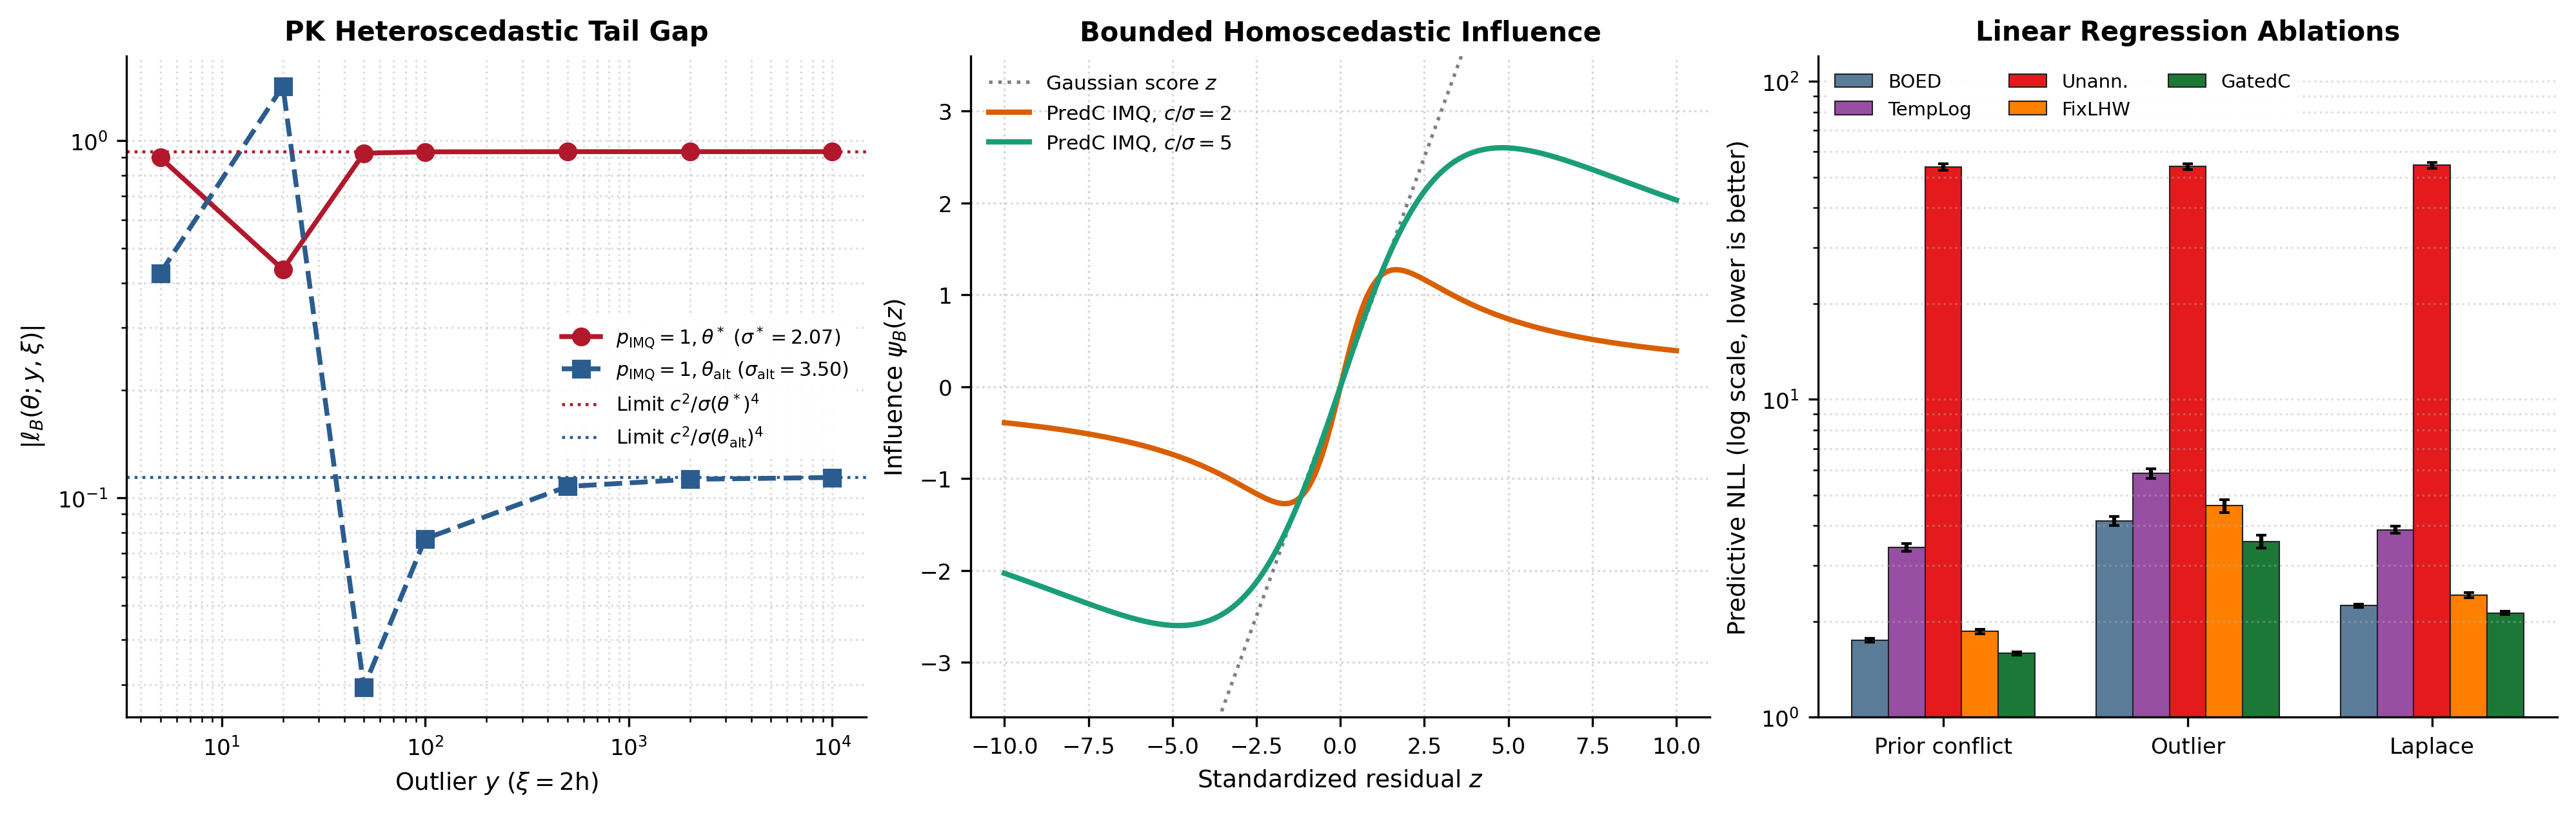
\includegraphics[width=0.98\textwidth]{figures/fig3_pk_and_ablations.png}
\caption{Left: pharmacokinetic tail loss at $\xi = 2\,\mathrm{h}$ ($p_{\mathrm{IMQ}} = 1$), converging to distinct asymptotes $c_{\mathrm{pk}}^2 / \sigma(\theta^*)^4 \approx 0.932$ and $c_{\mathrm{pk}}^2 / \sigma(\theta_{\mathrm{alt}})^4 \approx 0.114$ (\cref{thm:heteroscedastic}). Center: bounded influence $\psi_B(z)$ for PredC IMQ-WSM at $c/\sigma \in \{2, 5\}$ vs.\ Gaussian score $z$ (\cref{prop:stein_fisher}). Right: linear regression NLL ablations on logarithmic scale ($R=270$), showing unannealed PredC collapse ($\mathrm{NLL} \approx 54$) vs.\ annealed GatedC ($1.59, 3.57, 2.13$).}\label{fig:pk_ablation}
\end{figure}

\begin{table}[t]
\centering
\scriptsize
\setlength{\tabcolsep}{0.45pt}
\caption{Full ablation and baseline comparison across benchmarks (predictive MMD and NLL with unpaired standardized effect $z = z_{\mathrm{uSE}}$ vs.\ BOED in parentheses).}\label{tab:ablations}
\begin{tabular}{@{}l@{\hspace{3pt}}cccccc@{}}
\toprule
Method & \multicolumn{2}{c}{\texttt{none} / conf.} & \multicolumn{2}{c}{\texttt{outlier}} & \multicolumn{2}{c}{\texttt{error-dist} / \texttt{laplace}} \\
\cmidrule(lr){2-3}\cmidrule(lr){4-5}\cmidrule(lr){6-7}
& MMD ($z$) & NLL ($z$) & MMD ($z$) & NLL ($z$) & MMD ($z$) & NLL ($z$) \\
\midrule
\multicolumn{7}{@{}l}{\textbf{Location Finding ($d=4, R=90$)}} \\
\texttt{BOED} & $0.0106$ (ref) & $0.7573$ (ref) & $0.0498$ (ref) & $0.8837$ (ref) & $0.0501$ (ref) & $1.5131$ (ref) \\
\texttt{Fixed\_LHW} & $0.0109$ ($+0.26$) & $0.7589$ ($+0.41$) & $0.0206$ ($-9.97$) & $0.7871$ ($-9.87$) & $0.0493$ ($-1.23$) & $1.5060$ ($-1.80$) \\
\texttt{Barlas\_ExpDecay} & $0.0152$ ($+2.53$) & $0.7726$ ($+2.65$) & $0.0288$ ($-6.79$) & $0.8139$ ($-6.74$) & $0.0580$ ($+7.19$) & $1.5663$ ($+8.43$) \\
\texttt{GatedC\_G\_LHW} & $0.0116$ ($+0.78$) & $0.7608$ ($+0.84$) & $0.0189$ ($-10.75$) & $0.7808$ ($-10.71$) & $0.0486$ ($-2.23$) & $1.4994$ ($-3.11$) \\
\midrule
\multicolumn{7}{@{}l}{\textbf{Bayesian Linear Regression ($R=270$)}} \\
\texttt{BOED} & $0.1178$ (ref) & $1.7489$ (ref) & $0.6134$ (ref) & $4.1459$ (ref) & $0.1215$ (ref) & $2.2418$ (ref) \\
\texttt{Tempered\_LogLoss} & $0.5266$ ($+17.60$) & $3.4219$ ($+15.96$) & $0.8109$ ($+5.66$) & $5.8426$ ($+6.83$) & $0.4791$ ($+17.24$) & $3.8853$ ($+15.30$) \\
\texttt{Fixed\_LHW} & $0.1546$ ($+3.99$) & $1.8624$ ($+2.82$) & $0.5796$ ($-1.03$) & $4.6254$ ($+1.88$) & $0.1710$ ($+4.42$) & $2.4228$ ($+3.43$) \\
\texttt{Unannealed\_GatedC} & $1.3462$ ($+178.5$) & $53.7189$ ($+43.4$) & $1.3460$ ($+36.59$) & $53.9153$ ($+40.4$) & $1.3140$ ($+152.3$) & $54.4539$ ($+44.4$) \\
\texttt{Barlas\_Transf.} & $0.9365$ ($+21.53$) & $49.8138$ ($+20.16$) & $1.0744$ ($+13.21$) & $51.5760$ ($+19.91$) & $0.9377$ ($+22.48$) & $50.5509$ ($+20.51$) \\
\texttt{Barlas\_Regr.} & $0.8242$ ($+20.15$) & $15.7792$ ($+17.11$) & $0.9191$ ($+7.56$) & $14.6278$ ($+14.41$) & $0.7842$ ($+19.64$) & $16.9634$ ($+16.61$) \\
\texttt{GatedC\_G\_LHW} & $0.0634$ ($-7.97$) & $1.5897$ ($-5.09$) & $0.4212$ ($-6.47$) & $3.5685$ ($-2.65$) & $0.0828$ ($-4.62$) & $2.1255$ ($-2.97$) \\
\midrule
\multicolumn{7}{@{}l}{\textbf{Nonlinear Radial-Sinusoidal ($R=90$)}} \\
\texttt{BOED} & $0.0177$ (ref) & $0.5527$ (ref) & $0.2507$ (ref) & $1.4908$ (ref) & $0.1784$ (ref) & $3.2916$ (ref) \\
\texttt{Fixed\_LHW} & $0.0159$ ($-0.76$) & $0.5475$ ($-0.77$) & $0.1025$ ($-7.20$) & $0.8776$ ($-5.84$) & $0.1826$ ($+0.72$) & $3.2644$ ($-0.43$) \\
\texttt{Tempered\_LogLoss} & $0.0227$ ($+0.79$) & $0.5775$ ($+0.93$) & $0.1828$ ($-3.43$) & $1.0613$ ($-4.90$) & $0.1520$ ($-5.42$) & $2.8652$ ($-7.86$) \\
\texttt{GatedC\_G\_LHW} & $0.0140$ ($-1.80$) & $0.5416$ ($-1.91$) & $0.0988$ ($-7.84$) & $0.8276$ ($-7.81$) & $0.1473$ ($-5.83$) & $2.7646$ ($-9.20$) \\
\bottomrule
\end{tabular}
\end{table}

The ablation study (\cref{fig:pk_ablation}(c) and \cref{tab:ablations}) demonstrates why every component of GatedC G-LHW is indispensable. Dropping continuation (\texttt{Unannealed\_GatedC}) collapses completely ($\mathrm{NLL} \approx 54$). Dropping the conflict/dispersion gates (\texttt{Fixed\_LHW}) fails under conflicted regression ($+1.88$ to $+3.43$ NLL uSE) and under severe Nonlinear overdispersion ($+0.72$ MMD uSE). Replacing PredC IMQ-WSM by log-loss tempering (\texttt{Tempered\_LogLoss}) catastrophically degrades regression under all scenarios ($+6.83$ to $+15.96$ NLL uSE) and achieves smaller outlier gains than GatedC on Nonlinear ($-3.43$ vs.\ $-7.84$ MMD uSE). Barlas's fixed exponential schedule degrades well-specified and \texttt{error-dist} Location Finding ($+2.65$ and $+8.43$ NLL uSE) and collapses on conflicted regression ($+14.41$ to $+20.51$ NLL uSE across \texttt{Barlas\_Regr.} and \texttt{Barlas\_Transf.}). Ablations in \cref{tab:ablations} are grouped by architecture relevance: \texttt{Unannealed\_GatedC} and \texttt{Barlas\_Regr.} isolate linear-regression AnnealedPredC continuation, \texttt{Barlas\_ExpDecay} and \texttt{Barlas\_Transf.} apply the identical published decay schedule across SMC Location Finding and Linear Regression, and \texttt{Tempered\_LogLoss} isolates pure dispersion-tempered log-likelihood across continuous regression and nonlinear SMC.

\section{Scope, Limitations, and Open Questions}\label{sec:scope}

Our theory explicitly bounds its own validity domain:
\begin{enumerate}[label=\arabic*.]
\item \textbf{Heteroscedastic and design-varying noise.} Scalar PredC IMQ-WSM relies on homoscedastic, $\xi$-constant noise ($\rho_\theta, \rho_\xi \le 10^{-6}$). Extending calibration to variance-heteroscedastic pharmacokinetic simulators requires either weighted score matching defined over natural Riemannian coordinates ($\mathrm{d}z = \mathrm{d}y / \sigma_\theta(\xi)$) or variance-stabilizing transformations rather than raw $y$-space IMQ weights; we leave calibrated score-matching BOED on heteroscedastic models as a sharp open problem.
\item \textbf{Engineering constants vs.\ minimax optimality.} While $\omega_0(c) = \sigma^2 H_B/J_B$ is uniquely determined by multivariate Stein--Godambe geometry, the gating quantiles $(0.85, 0.95)$, conflict midpoint scales $(4, 16)$, floor $0.25$, and warmup $p+2$ are fixed engineering choices shown empirically effective, not proved minimax-optimal across arbitrary loss families.
\item \textbf{Asymptotic prior conflict behavior.} Because $\phi(\hat{\Delta}_0^2)$ evaluates conflict against the fixed initial prior $\Sigma_0$, $\gamma_\infty = \phi(\Delta_{0,\infty}^2)\tau_\infty$ remains in $(1, 2]$ when $\theta^* \neq \mu_0$ even at large $T$, accelerating bias removal at the cost of tighter asymptotic credible intervals; decaying conflict sensitivity as $t \to \infty$ is an immediate extension if exact large-$T$ frequentist interval width is desired.
\end{enumerate}

\section*{Declarations}

\subsection*{Acknowledgments}
None beyond the public open-source dependencies (\texttt{PyTorch}, \texttt{SciPy}, \texttt{python-flint}) and reference codebase~\cite{barlas2025gboed}.

\subsection*{Funding}
This research received no external grant or institutional funding.

\subsection*{Conflict of Interest}
The author declares no conflict of interest.

\subsection*{Data and Code Availability}
Complete source code, unit tests (\nolinkurl{tests/test_invariants.py}), 50-digit \texttt{python-flint} verification (\nolinkurl{scripts/verify_theorem_and_barlas_audit.py}), GPU benchmark suite (\nolinkurl{scripts/run_all_benchmarks.py}), and raw JSON logs (\nolinkurl{results/audit_results.json} and \nolinkurl{results/benchmark_results.json}) accompany the project workspace (\texttt{ORCID: 0009-0007-3678-0810}).

\section*{Use of AI and Computational Verification}
The author's main contributions are the identification of the homoscedastic vs.\ heteroscedastic tail gap separation for PredC IMQ-WSM, the design-time LHW--Stein Fisher calibration principle paired with $\chi^2$ dispersion gating and conflict relief, and the Bayesian scale continuation architecture eliminating unprincipled robust regressors. The author prompted Google Gemini to work through analytical derivations interactively, write the \texttt{python-flint} arbitrary-precision checks, vectorized CUDA SMC/Gibbs-EIG scripts, and unit tests, and draft the manuscript text; every proof, theorem constant, GPU run, and test suite was independently inspected and verified computationally against JSON logs and PDF renders.

\appendix

\section{Complete Analytical Proofs}\label{app:proofs}

\begin{proof}[Proof of \cref{thm:heteroscedastic}]
Write $r = y - \hat{\mu}$, $u(r) = 1 + r^2/c(\xi)^2$, so $m^2 = u^{-p}$ and $(m^2)' = -2p r\,c^{-2} u^{-p-1}$ with $p = p_{\mathrm{IMQ}} > 0$. Expanding~\eqref{eq:predc_loss_def} with $s_\theta = (\mu_\theta - y)/\sigma_\theta^2$ and $\partial_y s_\theta = -\sigma_\theta^{-2}$ yields
\[
\ell_B(\theta; y, \xi)
= \frac{r + \hat{\mu} - \mu_\theta}{\sigma_\theta^4}\Bigl[u^{-p}(r + \hat{\mu} - \mu_\theta) + \frac{4p\sigma_\theta^2 r}{c^2}u^{-p-1}\Bigr] - \frac{2}{\sigma_\theta^2}u^{-p}.
\]
In the regime $|r| \to \infty$ at fixed $\theta, \xi, \hat{\mu}$, $u(r) = r^2 c^{-2}(1 + \mathcal{O}(r^{-2}))$, so $r^2 u(r)^{-p} = c^{2p} |r|^{2-2p}(1 + \mathcal{O}(r^{-2}))$.
For (a), when $\sigma_\theta(\xi) \equiv \sigma$ is constant in $(\theta, \xi)$, all $(\mu_{\theta_1}-\mu_{\theta_2})$-independent terms ($r^2 u^{-p}\sigma^{-4}$, $4p r^2 u^{-p-1}/(\sigma^2 c^2)$, and $-2 u^{-p}\sigma^{-2}$) cancel identically in $\ell_B(\theta_1; y, \xi) - \ell_B(\theta_2; y, \xi)$, leaving
\[
\ell_B(\theta_1; y, \xi) - \ell_B(\theta_2; y, \xi)
= -\frac{2(\mu_{\theta_1} - \mu_{\theta_2})}{\sigma^4}\,r\,u(r)^{-p} + \mathcal{O}\bigl(u(r)^{-p}\bigr) + \mathcal{O}\bigl(|r|\,u(r)^{-p-1}\bigr).
\]
Since $u(r)^{-p} = \mathcal{O}(|r|^{-2p}) \to 0$ and $|r|u(r)^{-p-1} = \mathcal{O}(|r|^{-2p-1}) \to 0$ for every $p > 0$, while $|r|u(r)^{-p} = c(\xi)^{2p}|r|^{1-2p}(1 + \mathcal{O}(r^{-2}))$, the difference vanishes as $|y| \to \infty$ for all bounded $\mu_\theta(\xi)$ when $p > 1/2$ ($\Delta_\infty(\xi) = 0$). Whenever $\sup_{\theta_1,\theta_2}|\mu_{\theta_1}(\xi) - \mu_{\theta_2}(\xi)| > 0$, setting $p = 1/2$ leaves the finite nonzero asymptote $2c(\xi)\sigma^{-4}\sup_{\theta_1,\theta_2}|\mu_{\theta_1}(\xi) - \mu_{\theta_2}(\xi)| > 0$, whereas $0 < p < 1/2$ yields $1 - 2p > 0$ and hence $\Delta_\infty(\xi) = +\infty$.
For (b), setting $p = 1$ gives $r^2 u(r)^{-1} = c(\xi)^2 + \mathcal{O}(r^{-2})$ while $r u^{-1} = \mathcal{O}(r^{-1})$ and $u^{-1} = \mathcal{O}(r^{-2})$, leaving $\lim_{|y|\to\infty} \ell_B(\theta; y, \xi) = c(\xi)^2/\sigma_\theta(\xi)^4$. Taking the supremum over pairs $(\theta_1, \theta_2) \in \Theta^2$ yields $\Delta_\infty(\xi) = c(\xi)^2 (\sup_\theta \sigma_\theta(\xi)^{-4} - \inf_\theta \sigma_\theta(\xi)^{-4})$. In the PK model $\sigma_\theta(\xi) = (0.01\mu_\theta(\xi)^2 + 0.1)^{1/2} \ge \sqrt{0.1}$, $\sigma_\theta(\xi)^{-4} \in (0, 100]$, whence $0 < \Delta_\infty(\xi) \le 100 c(\xi)^2 < \infty$ whenever $\mu_\theta(\xi)^2$ is non-constant in $\theta$.
For (c), if $p > 1$, then $r^2 u^{-p} = \mathcal{O}(|r|^{2-2p}) \to 0$, giving $\Delta_\infty(\xi) = 0$; however, for any finite outlier $r = y - \hat{\mu} \neq 0$ with $u = 1 + r^2/c(\xi)^2 > 1$ (e.g., even when $\mu_{\theta_1}(\xi) = \mu_{\theta_2}(\xi) = \hat{\mu}$), $\ell_B(\theta; y, \xi) = u^{-p}[r^2 \sigma_\theta(\xi)^{-4} + 2(2pr^2/(c(\xi)^2 u) - 1)\sigma_\theta(\xi)^{-2}]$ is a non-degenerate quadratic in $\sigma_\theta(\xi)^{-2}$ with strictly positive leading coefficient $r^2 u^{-p} > 0$, preserving nonzero likelihood differences across $\sigma_{\theta_1}(\xi) \neq \sigma_{\theta_2}(\xi)$ on moderate outliers $|r| = \mathcal{O}(c(\xi))$.
\end{proof}

\begin{proof}[Proof of \cref{prop:stein_fisher}]
Differentiating~\eqref{eq:predc_loss_def} with respect to $\mu = \mu_\theta(\xi)$ while holding $\hat{\mu}, c, \sigma$ fixed gives
\[
\partial_\mu \ell_B(\mu; y; \hat{\mu}, c) = \frac{2 m(y)^2 (\mu - y)}{\sigma^4} + \frac{2 (m^2)'(y)}{\sigma^2}, \qquad
\partial_\mu^2 \ell_B(\mu; y; \hat{\mu}, c) = \frac{2 m(y)^2}{\sigma^4} > 0.
\]
This immediately proves (b). Since $(m^2)'$ is smooth, bounded, and decays like $|y|^{-2p_{\mathrm{IMQ}}-1}$, the product $y \mapsto m(y)^2 \phi_{\mu^*, \sigma}(y)$ vanishes at infinity and $(m^2)' \in L^1(\Ncal(\mu^*, \sigma^2))$. Integrating $\int_\R (m^2)'(y) \phi_{\mu^*, \sigma}(y)\,\dd y$ by parts~\cite{hyvarinen2005score} using $\partial_y \phi_{\mu^*, \sigma}(y) = -\frac{y-\mu^*}{\sigma^2}\phi_{\mu^*, \sigma}(y)$ gives $\E[(m^2)'(Y)] = \frac{1}{\sigma^2}\E[m(Y)^2(Y - \mu^*)]$, so at $\mu = \mu^*$:
\[
\E\bigl[\partial_\mu \ell_B(\mu^*; Y; \hat{\mu}, c)\bigr] = \frac{2}{\sigma^4}\E\bigl[m(Y)^2(\mu^* - Y)\bigr] + \frac{2}{\sigma^4}\E\bigl[m(Y)^2(Y - \mu^*)\bigr] = 0,
\]
proving (a) for arbitrary fixed $\hat{\mu} \in \R$. Setting $\hat{\mu} = \mu^*$ and $Y = \mu^* + \sigma Z$ with $Z \sim \Ncal(0,1)$ expresses $\partial_\mu \ell_B(\mu^*; \mu^* + \sigma Z) = -\frac{2}{\sigma^3}\psi_B(Z; r, p_{\mathrm{IMQ}})$, matching $H_B$ and $J_B$ in (b).

For (c), let $p = p_{\mathrm{IMQ}}$, $z = rw$, $u = 1 + w^2 \ge 1$. For large $|w|$, $\psi_B(rw) \sim r\,\mathrm{sgn}(w)|w|^{1-2p}$, which is bounded iff $1 - 2p \le 0 \iff p \ge 1/2$. Differentiating $\psi_B(rw) = r w (u^{-p} + 2p r^{-2} u^{-p-1})$ with respect to $w$ ($\dd u / \dd w = 2w = 2\sqrt{u-1}$) yields
\[
\frac{\dd \psi_B(rw)}{\dd w} = r\,u^{-p-2}\Bigl[(1 - 2p)u^2 + 2p\bigl(1 - (2p+1)r^{-2}\bigr)u + 4p(p+1)r^{-2}\Bigr].
\]
For $p = 1$, changing back via $u = 1 + w^2$ transforms the bracketed quadratic into $-(w^4 + 6r^{-2}w^2 - (1 + 2r^{-2})) = 0$, whose unique positive root is $w_*^2 = \sqrt{9r^{-4} + 2r^{-2} + 1} - 3r^{-2}$; at $w=0$ the derivative equals $r(1 + 2r^{-2}) > 0$ and as $w \to \infty$ the bracket becomes negative, confirming $w_*(r)$ is the global maximizer of $|\psi_B(rw)|$.
\end{proof}

\begin{proof}[Proof of \cref{cor:multivariate_lhw}]
Let $g_\theta(\xi_j) = \nabla_\theta \mu_\theta(\xi_j) \in \R^p$ and $K_\theta(\xi_j) = \nabla_\theta^2 \mu_\theta(\xi_j) \in \R^{p \times p}$. By the chain rule on~\eqref{eq:predc_loss_def},
\begin{align*}
\nabla_\theta \ell_B(\theta; Y_j, \xi_j; \hat{\mu}, c) &= \partial_\mu \ell_B(\mu_\theta(\xi_j); Y_j; \hat{\mu}, c)\,g_\theta(\xi_j), \\
\nabla_\theta^2 \ell_B(\theta; Y_j, \xi_j; \hat{\mu}, c) &= \partial_\mu^2 \ell_B\,g_\theta g_\theta^\top + \partial_\mu \ell_B\,K_\theta(\xi_j).
\end{align*}
Evaluate first at oracle centering $\hat{\mu} = \mu_{\theta^*}(\xi_j)$: because $\xi_j$ is $\mathcal{F}_{j-1}$-measurable and $Y_j \mid \mathcal{F}_{j-1} \sim \Ncal(\mu_{\theta^*}(\xi_j), \sigma^2)$, \cref{prop:stein_fisher}(a) gives $\E[\partial_\mu \ell_B(\mu_{\theta^*}(\xi_j); Y_j; \mu_{\theta^*}(\xi_j), c) \mid \mathcal{F}_{j-1}] = 0$ identically, while $\E[\partial_\mu^2 \ell_B \mid \mathcal{F}_{j-1}] = H_B(c/\sigma)/\sigma^4$ and $\E[(\partial_\mu \ell_B)^2 \mid \mathcal{F}_{j-1}] = J_B(c/\sigma)/\sigma^6$ for every $j$. Under $\|K_{\theta^*}(\xi)\|_{\mathrm{op}} \le K_\mu$ and $\|g_{\theta^*}(\xi)\|_2 \le L_\mu$, the centered curvature increments $\partial_\mu \ell_B\,K_{\theta^*}(\xi_j)$ form an $\mathcal{F}_j$-martingale difference sequence with uniformly bounded conditional second moment $\le (J_B(c/\sigma)/\sigma^6) K_\mu^2 < \infty$, and likewise $(\partial_\mu^2 \ell_B - H_B/\sigma^4)g_{\theta^*}g_{\theta^*}^\top$ and $((\partial_\mu \ell_B)^2 - J_B/\sigma^6)g_{\theta^*}g_{\theta^*}^\top$ are uniformly bounded $\mathcal{F}_j$-martingale differences for all $p_{\mathrm{IMQ}} \ge 1/2$ (by \cref{prop:stein_fisher}(c) and $|\partial_\mu^2 \ell_B| \le 2/\sigma^4$). Hence the $L^2$ martingale law of large numbers yields oracle averages $\bar{H}_T^{\mathrm{ora}}(c) = \frac{H_B(c/\sigma)}{\sigma^4}\bar{G}_T + o_p(1)$ and $\bar{J}_T^{\mathrm{ora}}(c) = \frac{J_B(c/\sigma)}{\sigma^6}\bar{G}_T + o_p(1)$. Moreover, holding $(y, \mu^*)$ fixed and differentiating with respect to $\hat{\mu}$ ($r = y - \hat{\mu}$) gives $\partial_{\hat{\mu}} \partial_\mu^2 \ell_B = -\frac{2}{\sigma^4}(m^2)'(r)$, $\partial_{\hat{\mu}} \partial_\mu \ell_B = \frac{2}{\sigma^4}[r(m^2)'(r) - (\mu^* - \hat{\mu})(m^2)'(r) - \sigma^2 (m^2)''(r)]$, and $\partial_{\hat{\mu}}[(\partial_\mu \ell_B)^2] = 2(\partial_\mu \ell_B)\partial_{\hat{\mu}}\partial_\mu \ell_B$. All three $\hat{\mu}$-derivatives are uniformly bounded over $y \in \R$ and $|\hat{\mu} - \mu_{\theta^*}(\xi_j)| \le 1$ whenever $p_{\mathrm{IMQ}} \ge 1/2$ (since $|r\,m(r)^2| \le C < \infty$ iff $p_{\mathrm{IMQ}} \ge 1/2$ while $|r(m^2)'(r)|$, $|(m^2)'(r)|$, $|(m^2)''(r)|$ are bounded for every $p_{\mathrm{IMQ}} > 0$). Thus substituting batch empirical centerings satisfying $\max_{1\le j\le T}|\hat{\mu}_{T,j} - \mu_{\theta^*}(\xi_j)| \to_p 0$ perturbs $\bar{H}_T(c)$ and $\bar{J}_T(c)$ deterministically by $o_p(1)$ without requiring $\hat{\mu}_{T,j}$ to be $\mathcal{F}_{j-1}$-measurable. Because both matrices are scalar multiples of the same $\bar{G}_T \succeq \lambda_{\min} I_p \succ 0$, $(\omega_0(c)\,\bar{H}_T(c))^{-1} = \bar{H}_T(c)^{-1}\bar{J}_T(c)\bar{H}_T(c)^{-1}(1+o_p(1))$ cancels $\bar{G}_T^{-1}$ completely and forces $\omega_0(c) = (H_B(c/\sigma)/J_B(c/\sigma))\sigma^2$.
\end{proof}

\begin{proof}[Proof of \cref{prop:prior_trap}]
Completing the square under linear mean $\mu_\theta(\xi_j) = \phi_j^\top \theta$ gives posterior precision $P_\tau = P_0 + \tau S_T$ and mean deviation $m_\tau - \theta^* = P_\tau^{-1} P_0(\mu_0 - \theta^*) + P_\tau^{-1} \sigma^{-2}\tau \sum_{j=1}^T \phi_j \varepsilon_j$. Taking expectation gives bias $b(\tau) = P_\tau^{-1} P_0(\mu_0 - \theta^*)$. Let $v = P_0^{1/2}(\mu_0 - \theta^*) \neq 0$ and $A = P_0^{-1/2} S_T P_0^{-1/2} \succ 0$; then $P_0^{1/2}b(\tau) = (I + \tau A)^{-1}v$. On an orthonormal eigenbasis $\{e_i\}$ of $A$ with eigenvalues $\lambda_i > 0$, $\|P_0^{1/2}b(\tau)\|_2^2 = \sum_i (1 + \tau\lambda_i)^{-2} \langle v, e_i\rangle^2$, which is strictly decreasing in $\tau > 0$ and amplifies individual eigencomponents by $(1+\lambda_i)/(1+\tau\lambda_i) \to \tau^{-1}$ (squared ratio $\to \tau^{-2}$) when $\tau\lambda_i \gg 1$, proving (a). Part (b) follows verbatim from $m(y_j; \phi_j^\top\mu_0, c)^2 = (1 + (y_j - \phi_j^\top\mu_0)^2/c^2)^{-p_{\mathrm{IMQ}}}$ with $p_{\mathrm{IMQ}}=1, c=2\sigma, |y_j-\phi_j^\top\mu_0|=30\sigma$.
\end{proof}

\begin{proof}[Proof of \cref{thm:conflict_floor}]
In 1D, $P_{\tau} = \sigma_0^{-2} + \tau T \sigma^{-2} = \sigma^{-2}(r_0 + \tau T) = (u\sigma^2)^{-1}$. Because $r_0 u + \tau T u = 1$,
\[
\mu_{\mathrm{post},\tau} - \theta^* = r_0 u(\mu_0 - \theta^*) + (1 - r_0 u)(\bar{Y} - \theta^*).
\]
Since $\bar{Y} \sim \Ncal(\theta^*, \kappa\sigma^2 / T)$ independently of $Y_{\mathrm{true}} \sim \Ncal(\theta^*, \kappa\sigma^2)$ and $(r_0 u)^2(\mu_0-\theta^*)^2 = r_0^2 u^2 \sigma_0^2 \Delta_0^2 = r_0 \Delta_0^2 u^2 \sigma^2$, taking $\E[(\mu_{\mathrm{post},\tau} - \theta^*)^2] = \sigma^2(r_0 \Delta_0^2 u^2 + (1-r_0 u)^2 \kappa / T)$. Given data, $Y_{\mathrm{pred}} \sim \Ncal(\mu_{\mathrm{post},\tau}, \sigma^2(1+u))$, yielding Gaussian predictive density NLL $\frac{1}{2}\log(2\pi\sigma^2(1+u)) + \frac{(Y_{\mathrm{true}} - \mu_{\mathrm{post},\tau})^2}{2\sigma^2(1+u)}$. Taking total expectation over $(\bar{Y}, Y_{\mathrm{true}})$ adds $\kappa\sigma^2$ to residual MSE, yielding~\eqref{eq:exact_nll_1d} and~\eqref{eq:exact_mse_1d}. Differentiating~\eqref{eq:exact_nll_1d} with respect to $u$ at $u=0$ by the quotient rule ($\frac{1}{2}(1) + \frac{(-2r_0\kappa/T)\cdot 2 - \kappa(1+1/T)\cdot 2}{4}$) yields $\frac{1-\kappa}{2} - \frac{\kappa(1+2r_0)}{2T}$; differentiating~\eqref{eq:exact_mse_1d} at $u=0$ yields $\sigma^2(1 - 2r_0\kappa/T)$.
\end{proof}

\begin{proof}[Proof of \cref{prop:chi2_domination}]
Conditional on fixed designs $\xi_{1:t}$ ($\mathrm{rank}(\Phi_{1:t}) = p$), write $Y = \Phi_{1:t} \theta^* + \varepsilon$ with $\varepsilon \sim \Ncal(0, \sigma^2 I_t)$. For $\hat{\theta}_{\mathrm{OLS}} = (\Phi_{1:t}^\top\Phi_{1:t})^{-1}\Phi_{1:t}^\top Y$, the residual vector is $e = Y - \Phi_{1:t}\hat{\theta}_{\mathrm{OLS}} = (I_t - H)\varepsilon$, where $H = \Phi_{1:t}(\Phi_{1:t}^\top\Phi_{1:t})^{-1}\Phi_{1:t}^\top$ is an orthogonal projection of rank $p$. Hence $I_t - H$ is an orthogonal projection of rank $t - p$, so $\sigma^{-2}\|e\|_2^2 \sim \chi^2_{t-p}$ identically. For any (possibly data-dependent) $\hat{\Sigma}_t \succeq 0$, every denominator satisfies $\sigma^2 + \phi_j^\top\hat{\Sigma}_t\phi_j \ge \sigma^2 > 0$ pointwise, giving the pathwise upper bound
\[
S_t^{\mathrm{pred}} = \sum_{j=1}^t \frac{e_j^2}{\sigma^2 + \phi_j^\top\hat{\Sigma}_t\phi_j} \le \frac{\|e\|_2^2}{\sigma^2} \sim \chi^2_{t-p}.
\]
Because adding $p$ independent squared standard normals preserves tail ordering ($\chi^2_{t-p} \preceq_{\mathrm{st}} \chi^2_t$), we obtain $\Prob(S_t^{\mathrm{pred}} > x \mid \xi_{1:t}) \le \Prob(\chi^2_{t-p} > x) \le \Prob(\chi^2_t > x)$ for every $x \ge 0$. Under prior shrinkage $\hat{\theta}_t - \hat{\theta}_{\mathrm{OLS}} = \mathcal{O}_p(\Delta_0 t^{-1})$ with $\|\phi_j\|_2 \le L_\mu$ and $\max_{1\le j\le t}\hat{\sigma}_{\mathrm{ep},j}^2 = \mathcal{O}_p(t^{-1})$, set $b = \Phi_{1:t}(\hat{\theta}_{\mathrm{OLS}} - \hat{\theta}_t)$ ($\|b\|_2 \le \sqrt{t} L_\mu \|\hat{\theta}_{\mathrm{OLS}} - \hat{\theta}_t\|_2 = \mathcal{O}_p(\Delta_0 t^{-1/2})$). Expanding $(\sigma^2 + \hat{\sigma}_{\mathrm{ep},j}^2)^{-1} = \sigma^{-2} - \hat{\sigma}_{\mathrm{ep},j}^2 \sigma^{-2}(\sigma^2 + \hat{\sigma}_{\mathrm{ep},j}^2)^{-1}$ in $Y_j - \phi_j^\top\hat{\theta}_t = e_j + b_j$ and invoking exact OLS orthogonality $e^\top b = e^\top\Phi_{1:t}(\hat{\theta}_{\mathrm{OLS}} - \hat{\theta}_t) = 0$, the leading cross-term vanishes identically, leaving Cauchy--Schwarz residual bound $2\sum_{j=1}^t \frac{\hat{\sigma}_{\mathrm{ep},j}^2}{\sigma^2(\sigma^2+\hat{\sigma}_{\mathrm{ep},j}^2)} |e_j b_j| = \mathcal{O}_p(t^{-1})\|e\|_2\|b\|_2 = \mathcal{O}_p(\Delta_0 t^{-1})$ and squared bias excess $\le \sigma^{-2}\|b\|_2^2 = \mathcal{O}_p(\Delta_0^2 t^{-1})$, hence total unnormalized excess $\mathcal{O}_p((\Delta_0^2 + \Delta_0)/t)$.
\end{proof}

\begin{proof}[Proof of \cref{thm:gatedc_guarantees}]
\emph{(a) Rate envelope:} Write $d = \hat{\Delta}_0^2 \ge 0$. Because $\phi(d) = 1 + d^2/(d^2+256) \in [1, 2]$ and $\tau_{\min}(d) = 1 - 0.75/(1 + (d/4)^2) \in [0.25, 1]$ for all $d \ge 0$, every step satisfies $\tau_t \in [0.25, 1]$ (including warmup $\tau_t=1$) and $c_t \in \{2\sigma, 5\sigma\}$ with $\omega_0(5\sigma) < \omega_0(2\sigma)$ from \cref{tab:quadrature}. Multiplying $\omega_t = \omega_{0,t}\phi(d)\tau_t$ gives $[0.25\omega_0(5\sigma),\, 2\omega_0(2\sigma)]$.

\emph{(b) Gross-error bound:} Write $r_j = y_j - \hat{\mu}_j$ and $\delta_j = \mu_\theta(\xi_j) - \hat{\mu}_j$. Differentiating \eqref{eq:predc_loss_def} with respect to $\theta$ under $p_{\mathrm{IMQ}}=1$ gives
\[
\nabla_\theta \ell_B(\theta; y_j, \xi_j) = \frac{2}{\sigma^4}\Bigl[m_j^2 \delta_j + \sigma^2 (m^2)'_j - m_j^2 r_j\Bigr]\nabla_\theta \mu_\theta(\xi_j).
\]
Under $|r_j| \to \infty$, $m_j^2 = (1 + r_j^2/c_t^2)^{-1} \to 0$, $|(m^2)'_j| \le 3\sqrt{3}/(8 c_t)$, and $|r_j m_j^2| \le c_t / 2$; on compact $\Theta$ with bounded $|\delta_j| \le 2 M_\mu$ and $\|\nabla_\theta\mu_\theta(\xi_j)\|_2 \le L_\mu$, every factor of $\nabla_\theta \ell_B$ stays uniformly bounded as $|y_j| \to \infty$. When $\delta_j = 0$, the bracket equals $-\sigma\psi_B(r_j/\sigma; c_t/\sigma, 1)$, giving Euclidean gradient norm $\frac{2}{\sigma^3}|\psi_B(r_j/\sigma; c_t/\sigma, 1)|\,\|\nabla_\theta\mu_\theta(\xi_j)\|_2 \le \frac{2 L_\mu}{\sigma^3}\sup_z|\psi_B(z; 5, 1)| = \frac{2 L_\mu}{\sigma^3}(2.6019195361\dots)$. In the linear conjugate model of \cref{prop:conjugate_predc} with $P_0 \succ 0$, denote $b_{\mathrm{post}} = P_0\mu_0 + \frac{2\omega}{\sigma^4}\sum_{j=1}^t (m_j^2 y_j - \sigma^2 (m^2)'_j)\phi_j$. Because $m_1^2 y_1 = m_1^2 \hat{\mu}_1 + m_1^2 r_1$, every observation satisfies $|m_1^2 y_1 - \sigma^2 (m^2)'_1| \le |\hat{\mu}_1| + \frac{c}{2} + \frac{3\sqrt{3}\sigma^2}{8c}$. At fixed $(c, \omega)$, the resolvent identity
\[
m_{\mathrm{post}}^{\mathrm{corr}} - m_{\mathrm{post}}^{\mathrm{clean}}
= \bigl(P_{\mathrm{post}}^{\mathrm{corr}}\bigr)^{-1}\bigl(b_{\mathrm{post}}^{\mathrm{corr}} - b_{\mathrm{post}}^{\mathrm{clean}}\bigr)
+ \bigl(P_{\mathrm{post}}^{\mathrm{corr}}\bigr)^{-1}\bigl(P_{\mathrm{post}}^{\mathrm{clean}} - P_{\mathrm{post}}^{\mathrm{corr}}\bigr)m_{\mathrm{post}}^{\mathrm{clean}}
\]
together with $P_{\mathrm{post}}^{\mathrm{corr}} \succeq P_0$ and $0 \le m_1^2 \le 1$ yields
\[
\|m_{\mathrm{post}}(y_1) - m_{\mathrm{post}}^{\mathrm{clean}}\|_2 \le \|P_0^{-1}\|_{\mathrm{op}}\Bigl(\frac{2\omega}{\sigma^4}\Delta_{\mathrm{rhs}}\|\phi_1\|_2 + \frac{2\omega}{\sigma^4}\|\phi_1\|_2^2 \|m_{\mathrm{post}}^{\mathrm{clean}}\|_2\Bigr) < \infty,
\]
where $\Delta_{\mathrm{rhs}} = |m_1^2 y_1 - \sigma^2(m^2)'_1| + |m_{1,\mathrm{clean}}^2 y_{1,\mathrm{clean}} - \sigma^2(m^2)'_{1,\mathrm{clean}}|$ stays uniformly bounded over all $y_1 \in \R$. Even when moving $|y_1| \to \infty$ causes the gate to switch $(\omega_t, c_t)$ within the bounded rectangle $[\omega_{\min}, \omega_{\max}] \times \{2\sigma, 5\sigma\}$ of part~(a), summing the same bound over the fixed bulk $y_{2:t}$ and observation $y_1$ ensures $\|m_{\mathrm{post}}(y_1, y_{2:t})\|_2$ and hence $\|m_{\mathrm{post}}(y_1, y_{2:t}) - m_{\mathrm{post}}^{\mathrm{clean}}\|_2$ remain uniformly finite. Under annealed continuation, whenever strictly fewer than half of observations are corrupted (in particular $t \ge 3$ for any single outlier), $\mathrm{med}_j |y_j - \hat{\mu}_j^{(0)}|$ depends only on uncorrupted bulk quantiles, keeping $c_{\max}$ and every intermediate scale $\hat{\mu}_j^{(s)}$ uniformly bounded over $|y_1| \to \infty$~\cite{huber1964robust}.

\emph{(c) Consistency:} Fix either threshold branch $c \in \{2\sigma, 5\sigma\}$ and consider the centered loss difference $\Delta\ell_B(\theta; y, \xi; \hat{\mu}, c) = \ell_B(\theta; y, \xi; \hat{\mu}, c) - \ell_B(\theta^*; y, \xi; \hat{\mu}, c)$. Setting $r = y - \hat{\mu}$ and substituting $(\mu_\theta - y)^2 - (\mu_{\theta^*} - y)^2 = (\mu_\theta - \mu_{\theta^*})^2 + 2(\mu_\theta - \mu_{\theta^*})(\mu_{\theta^*} - \hat{\mu} - r)$ yields
\begin{align*}
\Delta\ell_B(\theta; y, \xi; \hat{\mu}, c)
&= \frac{m(r)^2}{\sigma^4}(\mu_\theta - \mu_{\theta^*})^2 \\
&\quad + \frac{2(\mu_\theta - \mu_{\theta^*})}{\sigma^4}\Bigl[m(r)^2(\mu_{\theta^*} - \hat{\mu}) - m(r)^2 r + \sigma^2 (m^2)'(r)\Bigr].
\end{align*}
Because $m(r)^2$, $m(r)^2 r$, and $(m^2)'(r)$ are uniformly bounded with bounded derivatives over all $r \in \R$ at $p_{\mathrm{IMQ}}=1$, while $|\mu_\theta(\xi) - \mu_{\theta^*}(\xi)|$ and $\|\nabla_\theta\mu_\theta(\xi)\|_2$ are bounded under (A1)--(A2), $\Delta\ell_B$ is uniformly bounded and uniformly Lipschitz in $(\theta, \hat{\mu})$ over $(y, \xi) \in \R \times \Xcal$, requiring no moment conditions on $Y_j$. By (A3), replacing $\hat{\mu}_{t,j}$ with $\mu_{\theta^*}(\xi_j)$ shifts $t^{-1}\sum_{j=1}^t \Delta\ell_B$ by $o_p(1)$ uniformly on $\Theta \times \{2\sigma, 5\sigma\}$. At $\hat{\mu} = \mu_{\theta^*}(\xi_j)$ with $Z_j = Y_j - \mu_{\theta^*}(\xi_j)$, the term $-m(Z_j)^2 Z_j + \sigma^2 (m^2)'(Z_j)$ is odd and bounded; under both $\varepsilon = 0$ (via \cref{prop:stein_fisher}(a)) and symmetric heavy-tailed $Q_{\mathrm{out},j}$ (via odd symmetry in (A4)), its conditional expectation given $\mathcal{F}_{j-1}$ vanishes identically. Consequently, writing $\bar{D}_t(\theta; c) = t^{-1}\sum_{j=1}^t \Delta\ell_B(\theta; Y_j, \xi_j; \mu_{\theta^*}(\xi_j), c)$, conditional expectation yields $\E[\Delta\ell_B(\theta; Y_j, \xi_j; \mu_{\theta^*}(\xi_j), c) \mid \mathcal{F}_{j-1}] = \sigma^{-4}\E[m(Z_j; c)^2 \mid \mathcal{F}_{j-1}](\mu_\theta(\xi_j) - \mu_{\theta^*}(\xi_j))^2$, while by bulk tightness (A4), $\E[m(Z_j; c)^2 \mid \mathcal{F}_{j-1}] \ge \eta_0(1 + R_0^2/(2\sigma)^2)^{-1} > 0$ uniformly over $j$ and $c \in \{2\sigma, 5\sigma\}$. Since centered martingale differences of $\Delta\ell_B$ are uniformly bounded and Lipschitz in $\theta$ over compact $\Theta$, Azuma--Hoeffding over a finite $\epsilon$-net yields $\sup_{\theta \in \Theta} |\bar{D}_t(\theta; c) - t^{-1}\sum_{j=1}^t \E[\Delta\ell_B(\theta; Y_j, \xi_j; \mu_{\theta^*}(\xi_j), c) \mid \mathcal{F}_{j-1}]| \to_p 0$ simultaneously on $c \in \{2\sigma, 5\sigma\}$. Combining this lower bound with Wald identifiability (A2) implies $\hat{\theta}_t^{\mathrm{GBOED}} \to_p \theta^*$. (Under asymmetric $\varepsilon$-contamination, bounded $\psi_B$ shifts the pseudo-true limit by $\mathcal{O}(\varepsilon)$ rather than diverging.)

\emph{(d) Godambe covariance:} By (A3), $\phi(\hat{\Delta}_0^2) \to_p \phi(\Delta_{0,\infty}^2)$, and when $S_T^{\mathrm{pred}}/T \to_p s_\infty \le 1$ we have $\chi^2_{T, 0.95}/T \to 1$: on the event $S_T^{\mathrm{pred}} \le \chi^2_{T, 0.95}$ the gate gives $\tau_T = 1$, and whenever $S_T^{\mathrm{pred}} > \chi^2_{T, 0.95}$ (possible when $s_\infty = 1$) $T/S_T^{\mathrm{pred}} \to_p 1$, so in all cases $\tau_T = \max(\tau_{\min}, \min(1, T/S_T^{\mathrm{pred}})) \to_p 1$ without requiring $c_T \in \{2\sigma, 5\sigma\}$ to converge to a single value. Applying \cref{cor:multivariate_lhw} simultaneously on both fixed branches $c \in \{2\sigma, 5\sigma\}$ with $\gamma_T = \phi(\hat{\Delta}_0^2)\tau_T \to_p \gamma_\infty \in [0.25, 2.0]$, observe that in $\nabla_\theta^2 \ell_B = \partial_\mu^2 \ell_B\,g_\theta g_\theta^\top + \partial_\mu \ell_B\,K_\theta$, both $|\partial_\mu^2 \ell_B| \le 2/\sigma^4$ and $|\partial_\mu \ell_B(\mu_\theta(\xi_j); Y_j; \hat{\mu}_{T,j}, c)|$ are uniformly bounded on $\Theta \times \Xcal \times \R \times \{2\sigma, 5\sigma\}$ at $p_{\mathrm{IMQ}} = 1$, while by (A2) $g_\theta(\xi)$ and $K_\theta(\xi)$ are uniformly bounded ($L_\mu, K_\mu$) and $\theta \mapsto K_\theta(\xi)$ is equicontinuous at $\theta^*$ uniformly over $\Xcal$. Together with part~(c) ($\hat{\theta}_T^{\mathrm{GBOED}} \to_p \theta^*$ simultaneously over $c \in \{2\sigma, 5\sigma\}$), this ensures uniform local Hessian convergence $\sup_{\|\theta - \theta^*\|_2 \le \delta_T,\, c \in \{2\sigma, 5\sigma\}} \|T^{-1}\sum_{j=1}^T \nabla_\theta^2 \ell_B(\theta; Y_j, \xi_j; \hat{\mu}_{T,j}, c) - \bar{H}_T(c)\|_{\mathrm{op}} = o_p(1)$ for every $\delta_T \to 0$, controlling the quadratic Taylor remainder around $\hat{\theta}_T^{\mathrm{GBOED}}$, while Wald identifiability (A2) and $\omega_T \ge 0.25\omega_0(5\sigma) > 0$ exponentially suppress outer tails off shrinking neighborhoods of $\theta^*$. Hence standard Laplace / Bernstein--von Mises expansion of the batch-reweighted Gibbs posterior~\cite{lyddon2019general} yields quadratic precision $T\omega_0(c_T)\gamma_T\bar{H}_T(c_T)(1 + o_p(1))$. Since $\omega_0(c_T)\bar{H}_T(c_T) = \bar{H}_T(c_T)\bar{J}_T(c_T)^{-1}\bar{H}_T(c_T)(1 + o_p(1))$ holds identically on both branches $c_T \in \{2\sigma, 5\sigma\}$, inverting gives $\Sigma_{\mathrm{Gibbs}, T} = \frac{1}{T\gamma_\infty}\bar{H}_T(c_T)^{-1}\bar{J}_T(c_T)\bar{H}_T(c_T)^{-1}(1 + o_p(1))$.
\end{proof}

\begin{proof}[Proof of \cref{prop:conjugate_predc}]
For linear mean $\mu_\theta(\xi_j) = \phi_j^\top \theta$, expanding~\eqref{eq:predc_loss_def} as a quadratic polynomial in $\theta$ and dropping $\theta$-independent scalars $r_j(\theta) = \phi_j^\top\theta - y_j$:
\[
\ell_B(\phi_j^\top\theta; y_j) = \frac{m_j^2}{\sigma^4}(\phi_j^\top\theta - y_j)^2 + \frac{2(m^2)'_j}{\sigma^2}(\phi_j^\top\theta) + \mathrm{const}_j.
\]
Grouping quadratic and linear terms inside the negative log-Gibbs potential $\frac{1}{2}(\theta-\mu_0)^\top P_0 (\theta-\mu_0) + \omega \sum_{j=1}^t \ell_B(\phi_j^\top\theta; y_j)$ gives exact quadratic Hessian $P_{\mathrm{post}} = P_0 + \frac{2\omega}{\sigma^4}\sum_{j=1}^t m_j^2 \phi_j \phi_j^\top$ and stationary point equation $P_{\mathrm{post}} m_{\mathrm{post}} = P_0\mu_0 + \frac{2\omega}{\sigma^4}\sum_{j=1}^t (m_j^2 y_j - \sigma^2 (m^2)'_j)\phi_j$.
\end{proof}

\begin{thebibliography}{99}

\bibitem{altamirano2024rcgp}
M.~Altamirano, F.-X.~Briol, and J.~Knoblauch,
\newblock Robust and conjugate Gaussian process regression,
\newblock \emph{Proceedings of the 41st International Conference on Machine Learning (ICML)}, PMLR \textbf{235} (2024), arXiv:2311.00463.

\bibitem{barlas2025gboed}
Y.~Z.~Barlas, S.~J.~Sloman, and S.~Kaski,
\newblock Robust experimental design via generalised Bayesian inference,
\newblock \emph{arXiv preprint} arXiv:2511.07671 (2025).

\bibitem{barp2019minimum}
A.~Barp, F.-X.~Briol, A.~Duncan, M.~Girolami, and L.~Mackey,
\newblock Minimum Stein discrepancy estimators,
\newblock \emph{Advances in Neural Information Processing Systems} \textbf{32} (2019), arXiv:1906.08283.

\bibitem{bissiri2016general}
P.~G.~Bissiri, C.~C.~Holmes, and S.~G.~Walker,
\newblock A general framework for updating belief distributions,
\newblock \emph{Journal of the Royal Statistical Society Series B: Statistical Methodology} \textbf{78} (2016), no.~5, 1103--1130, doi:10.1111/rssb.12158.

\bibitem{godambe1960optimum}
V.~P.~Godambe,
\newblock An optimum property of regular maximum likelihood estimation,
\newblock \emph{The Annals of Mathematical Statistics} \textbf{31} (1960), no.~4, 1208--1211, doi:10.1214/aoms/1177705693.

\bibitem{grunwald2017inconsistency}
P.~D.~Gr\"unwald and T.~van~Ommen,
\newblock Inconsistency of Bayesian inference for misspecified linear models, and a proposal for repairing it,
\newblock \emph{Bayesian Analysis} \textbf{12} (2017), no.~4, 1069--1103, doi:10.1214/17-BA1085.

\bibitem{huber1964robust}
P.~J.~Huber,
\newblock Robust estimation of a location parameter,
\newblock \emph{The Annals of Mathematical Statistics} \textbf{35} (1964), no.~1, 73--101, doi:10.1214/aoms/1177703732.

\bibitem{hyvarinen2005score}
A.~Hyv\"arinen,
\newblock Estimation of non-normalized statistical models by score matching,
\newblock \emph{Journal of Machine Learning Research} \textbf{6} (2005), 695--709.

\bibitem{jewson2022loss}
J.~Jewson and D.~Rossell,
\newblock General Bayesian loss function selection and the use of improper models,
\newblock \emph{Journal of the Royal Statistical Society Series B: Statistical Methodology} \textbf{84} (2022), no.~5, 1640--1665, doi:10.1111/rssb.12553.

\bibitem{knoblauch2022optimization}
J.~Knoblauch, J.~Jewson, and T.~Damoulas,
\newblock An optimization-centric view on Bayes' rule: Reviewing and generalizing variational inference,
\newblock \emph{Journal of Machine Learning Research} \textbf{23} (2022), no.~132, 1--109, arXiv:1904.02063.

\bibitem{laplante2025strcgp}
W.~Laplante, M.~Altamirano, A.~Duncan, J.~Knoblauch, and F.-X.~Briol,
\newblock Robust and conjugate spatio-temporal Gaussian processes,
\newblock \emph{Proceedings of the 42nd International Conference on Machine Learning (ICML)} (2025), arXiv:2502.02450.

\bibitem{lindley1956measure}
D.~V.~Lindley,
\newblock On a measure of the information provided by an experiment,
\newblock \emph{The Annals of Mathematical Statistics} \textbf{27} (1956), no.~4, 986--1005, doi:10.1214/aoms/1177728069.

\bibitem{lyddon2019general}
S.~P.~Lyddon, C.~C.~Holmes, and S.~G.~Walker,
\newblock General Bayesian updating and the loss-likelihood bootstrap,
\newblock \emph{Biometrika} \textbf{106} (2019), no.~2, 465--478, doi:10.1093/biomet/asz006.

\bibitem{overstall2020acebayes}
A.~M.~Overstall, D.~C.~Woods, and M.~Adamou,
\newblock acebayes: An {R} package for Bayesian optimal design of experiments via approximate coordinate exchange,
\newblock \emph{Journal of Statistical Software} \textbf{95} (2020), no.~13, 1--33, doi:10.18637/jss.v095.i13.

\bibitem{rainforth2024modern}
T.~Rainforth, A.~Foster, D.~R.~Ivanova, and F.~Bickford~Smith,
\newblock Modern Bayesian experimental design,
\newblock \emph{Statistical Science} \textbf{39} (2024), no.~1, 100--114, doi:10.1214/23-STS915.

\bibitem{wu2023comparison}
P.-S.~Wu and R.~Martin,
\newblock A comparison of learning rate selection methods in generalized Bayesian inference,
\newblock \emph{Bayesian Analysis} \textbf{18} (2023), no.~1, 105--132, doi:10.1214/21-BA1302.

\end{thebibliography}

\end{document}
